%======================================================================
\chapter{Assembly Instructions}
\label{ch: assemblyInstructions}
%======================================================================

This appendix explains how to assemble the robot from the individual components. Some useful tools to have on hand during the assembly are a 2.5mm Allen key, a pair of needlenose pliers, a wire stripper, a scissors, and an exacto knife. Follow the steps below to assemble the robot.

\vspace*{18pt}
\noindent
\begin{Large}\textbf{Instructions}\end{Large}

\begin{enumerate}[label = \textbf{Step \arabic*.}]
    \item Get a Budget Bot Chassis (Fig. \ref{fig:assemblyBudgetBot}). For this project, a fuse, power switch, and power indicator LED were added to the Budget Bot Chassis. Install a 2-cell LiPo battery inside the Budget Bot. Route the balance plug and battery output cable up through the center hole on top of the Budget Bot.
    \begin{figure}[H]
        \centering
        \includegraphics[width=3.6in]{figs/img/assembly/01-BudgetBot.png}
        \caption{Modified Budget Bot Chassis}
        \label{fig:assemblyBudgetBot}
    \end{figure}

    \item Install a BeagleBone Blue and a solderless breadboard on the Budget Bot using 6mm M3 screws (Fig. \ref{fig:bbblueInstallation}, red circles). Connect the battery's balance plug to the terminal on the BBBlue, and the power output to the breadboard (Fig. \ref{fig:bbblueInstallation}, green circles). Finally, insert the motor cables into the breadboard (Fig. \ref{fig:bbblueInstallation}, blue circle).
    \begin{figure}[H]
        \centering
        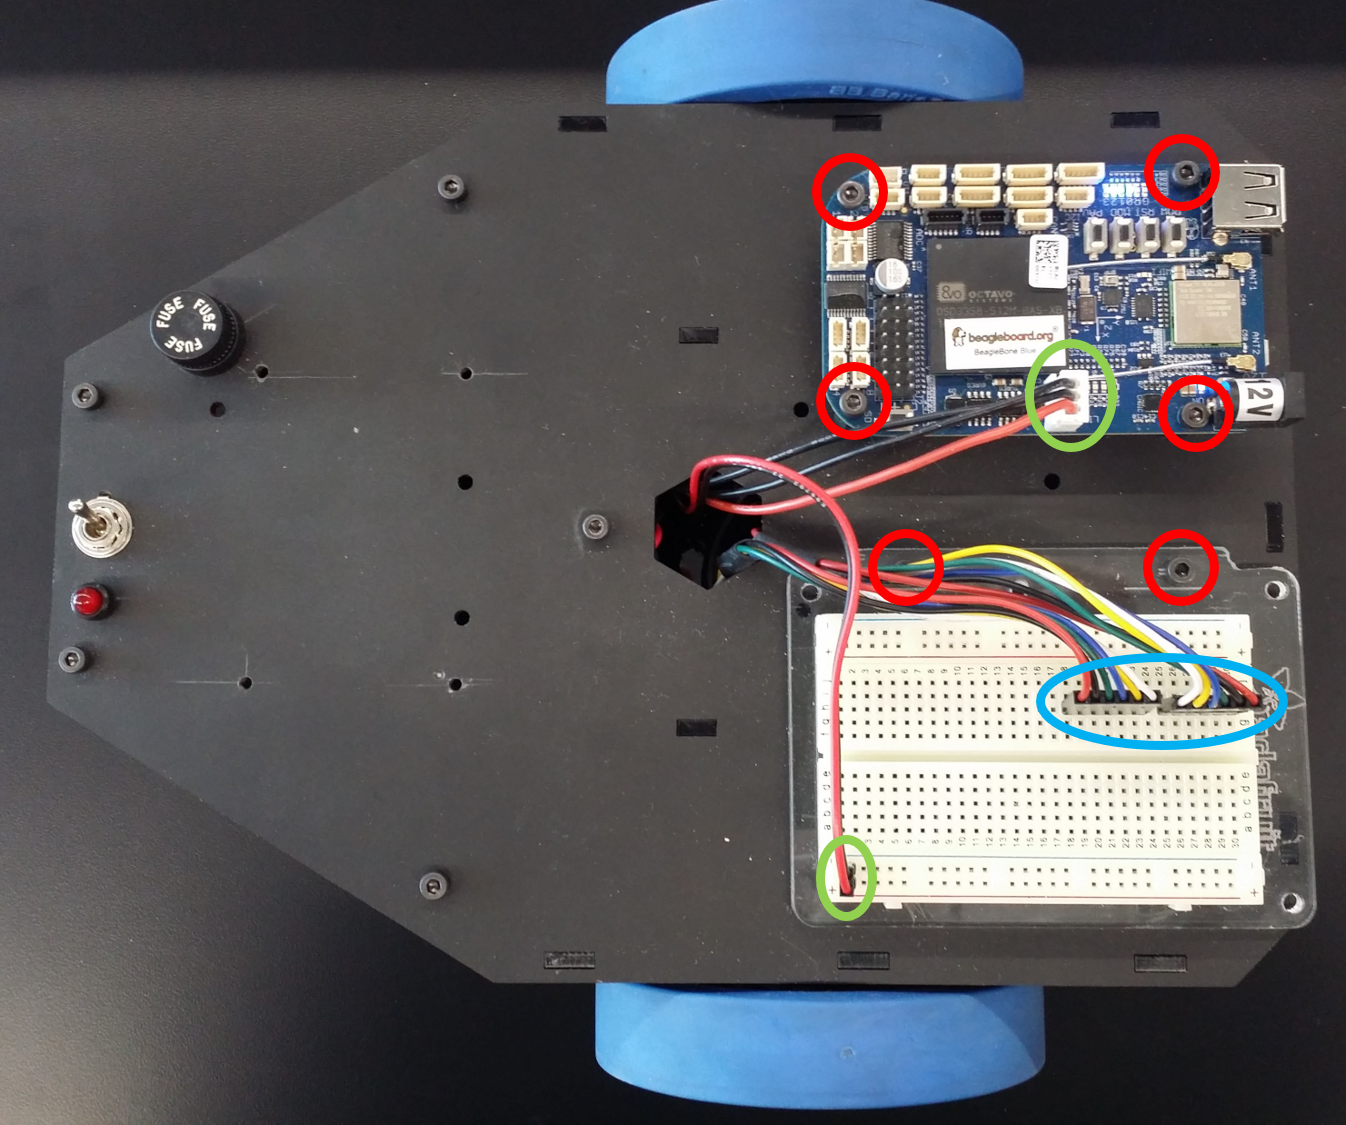
\includegraphics[width=3.6in]{figs/img/assembly/02-bbblueInstallation.png}
        \caption{BBBlue and Breadboard Installation}
        \label{fig:bbblueInstallation}
    \end{figure}

    \item Connect the motor terminals to the motor output channels on the BBBlue (left: ch1, right: ch2) using two 2-pin JST-ZH connectors. Connect the motor encoders to the encoder channels on the BBBlue (left: ch1, right: ch2) using two 4-pin JST-SH connectors (Fig. \ref{fig:motorWiring}).
    \begin{figure}[H]
        \centering
        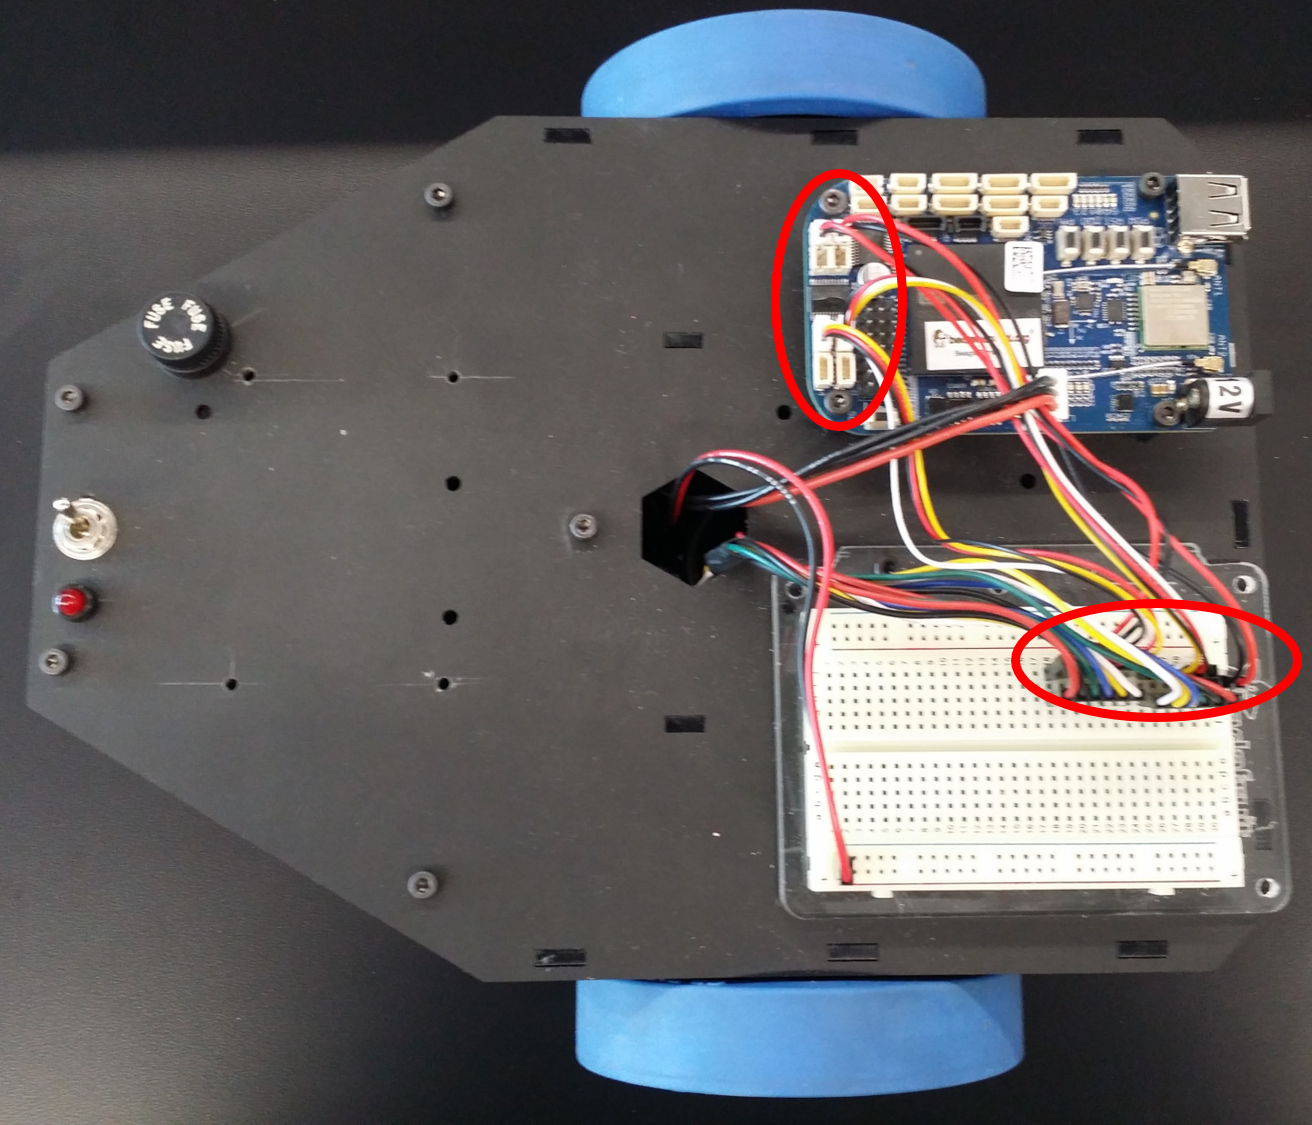
\includegraphics[width=3.6in]{figs/img/assembly/03-motorWiring.png}
        \caption{Motor Wiring}
        \label{fig:motorWiring}
    \end{figure}

    \item Prepare the stepper motor, the stepper motor bracket, four 6mm M3 screws, and four 8mm M3 screws (Fig. \ref{fig:stepperParts}).
    \begin{figure}[H]
        \centering
        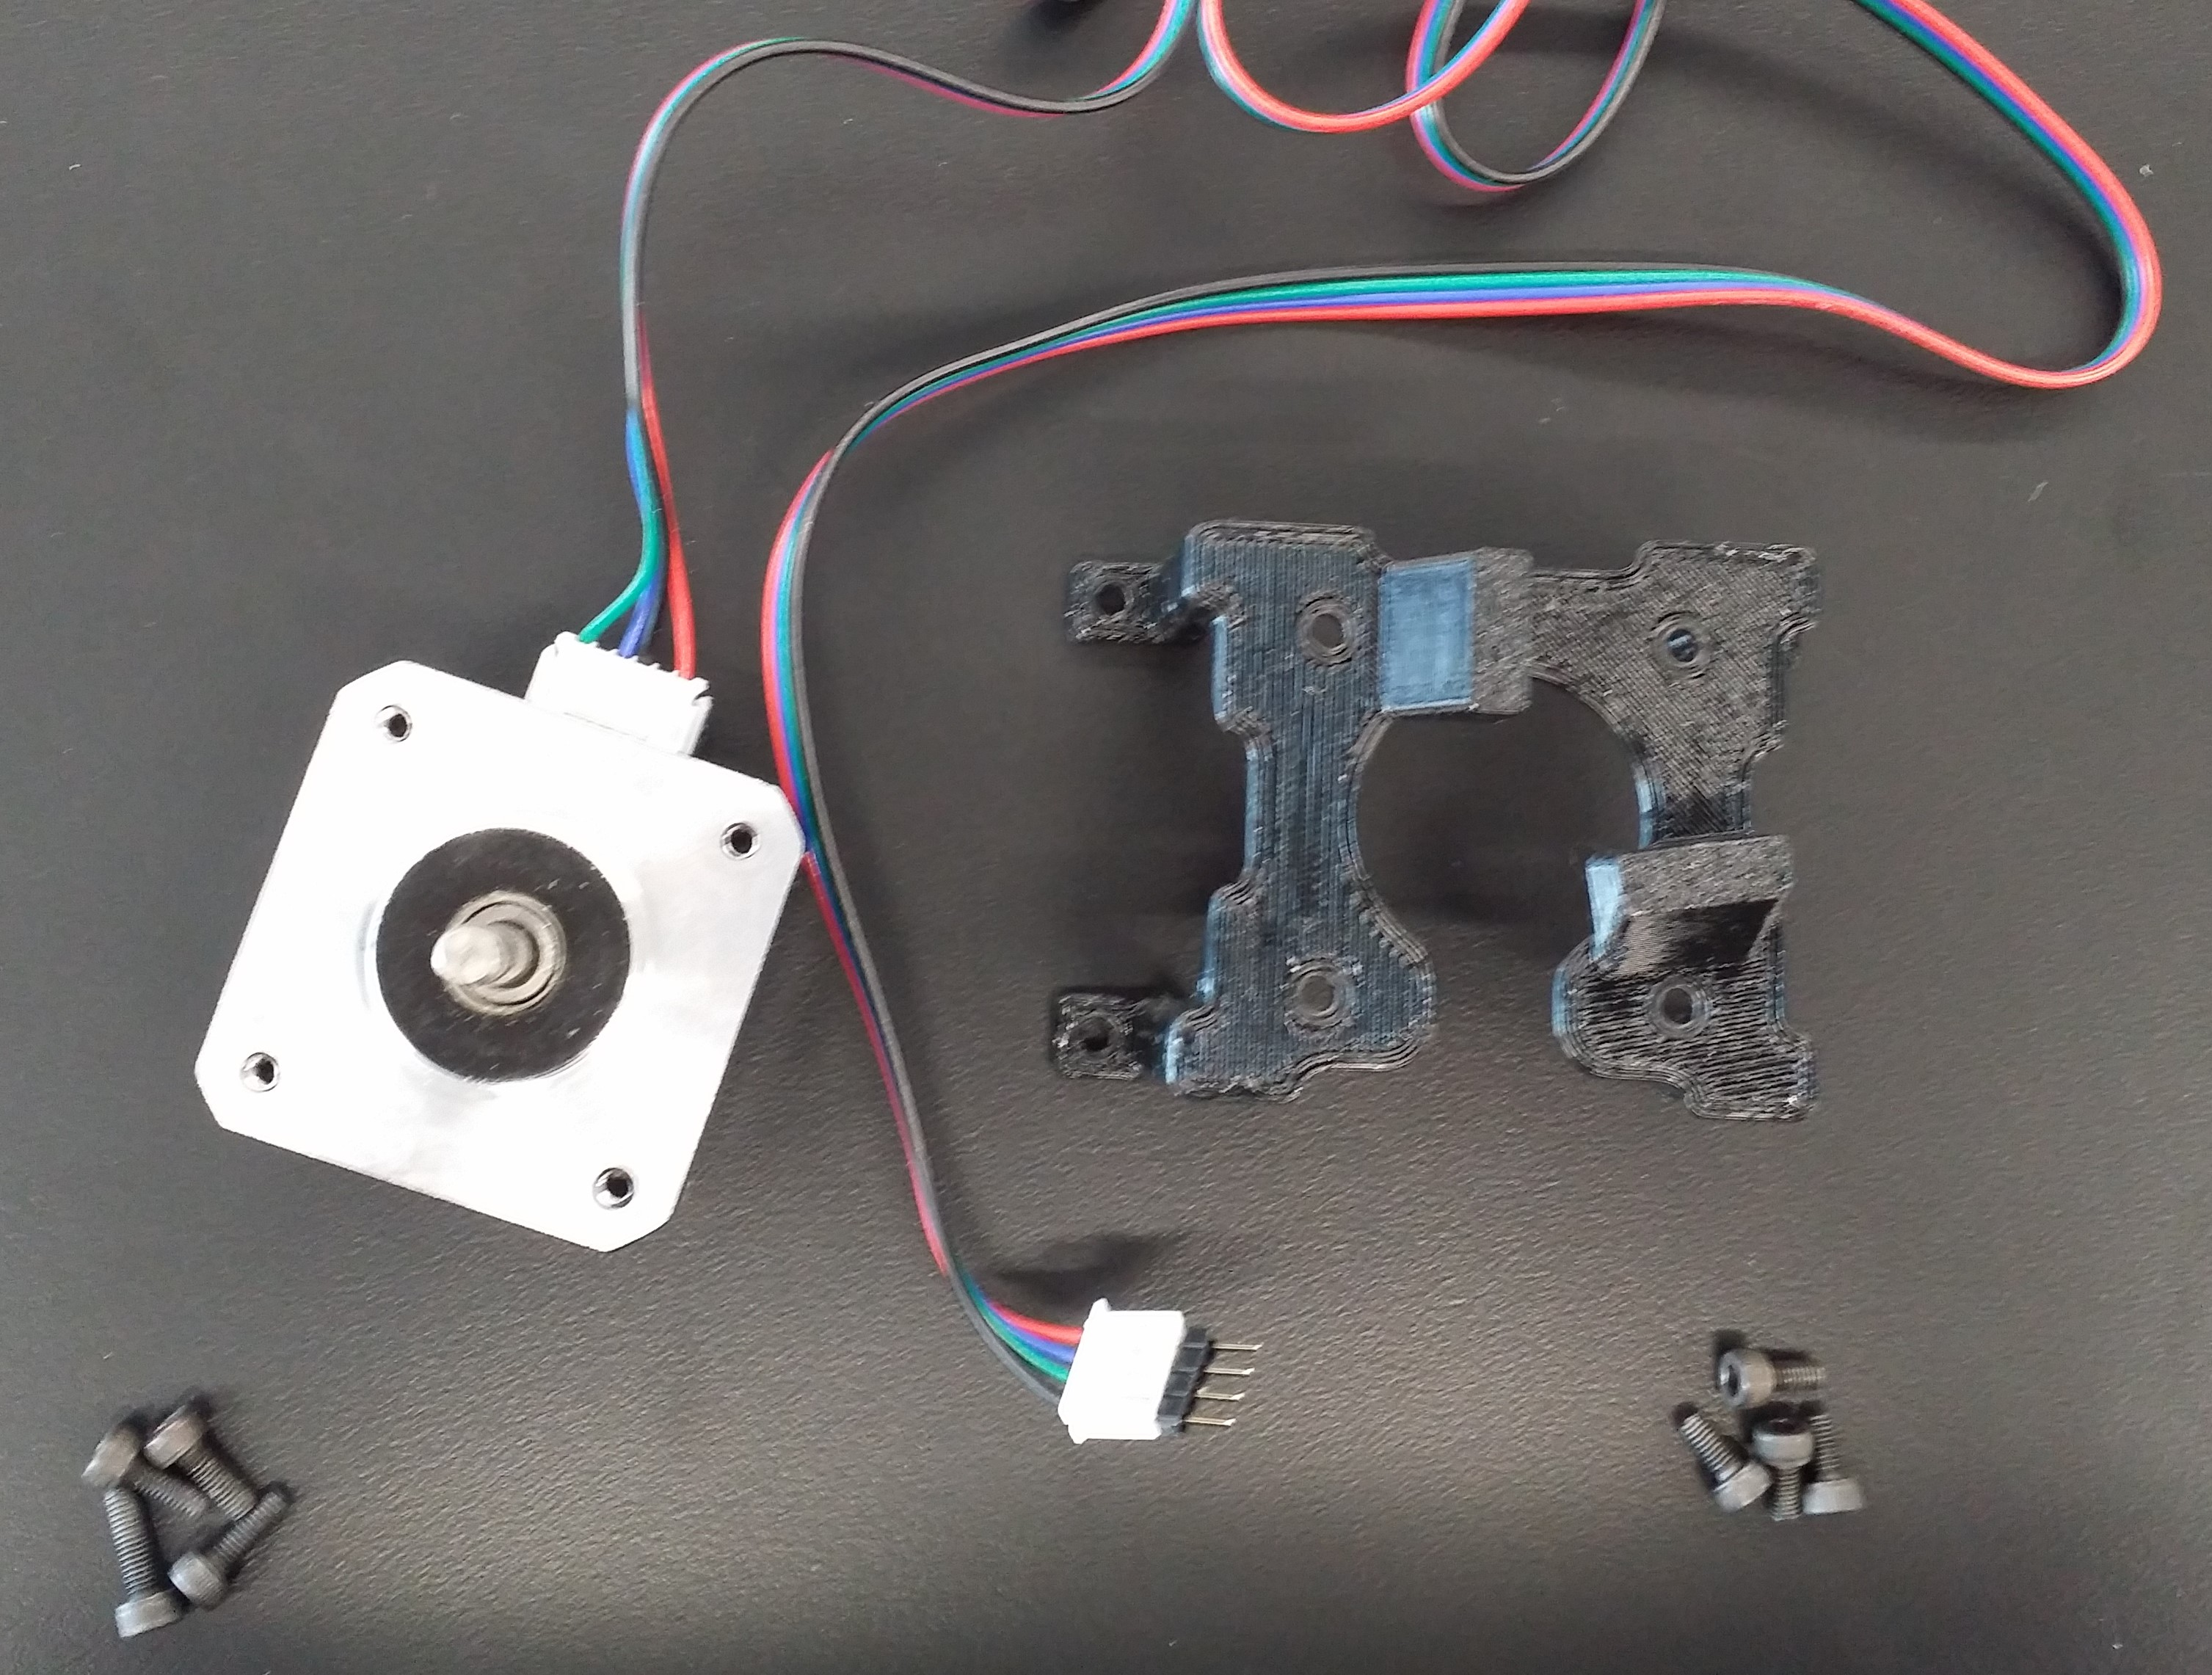
\includegraphics[width=4in]{figs/img/assembly/04-stepperParts.jpg}
        \caption{Stepper Motor Parts}
        \label{fig:stepperParts}
    \end{figure}

    \item Insert four 6mm M3 screws through the holes on the top of the bracket and secure the stepper motor to the stepper motor bracket by threading the screws into the holes in the stepper motor (Fig. \ref{fig:stepperAssembly}). Make sure the motor connector comes out on the side of the bracket with the notch.
    \begin{figure}[H]
        \centering
        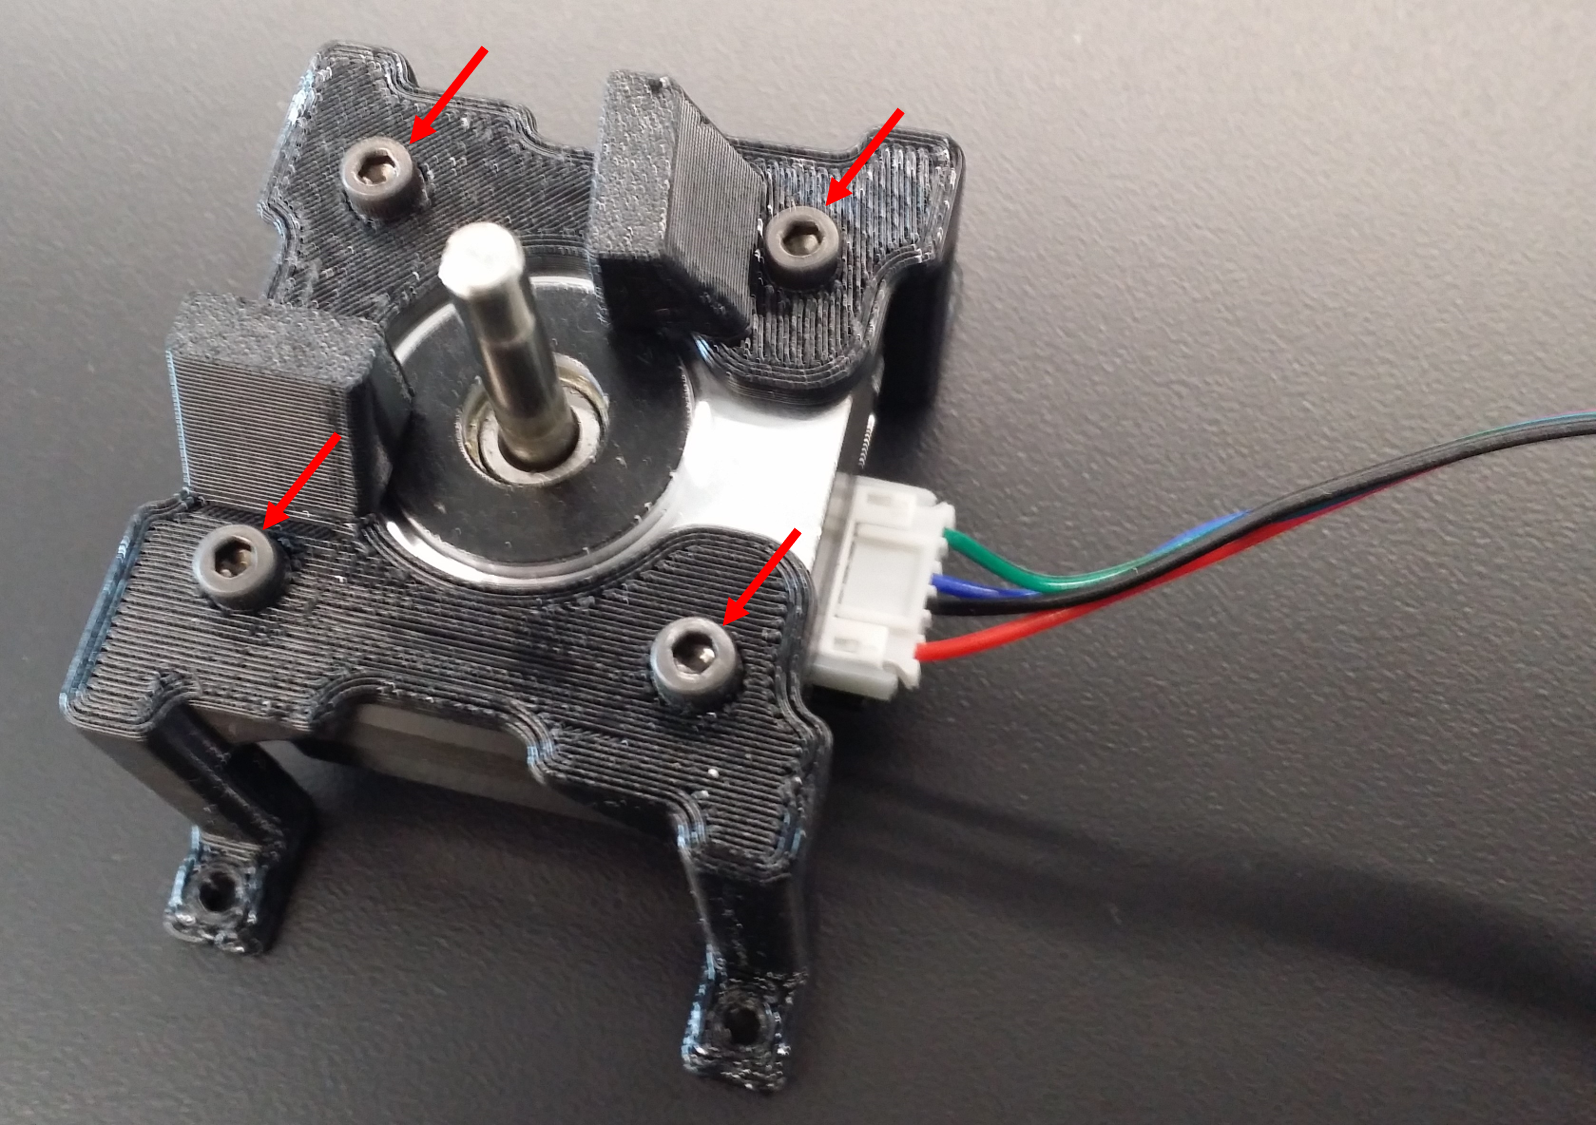
\includegraphics[width=4in]{figs/img/assembly/05-stepperAssembly.png}
        \caption{Mounting Stepper Motor onto Bracket}
        \label{fig:stepperAssembly}
    \end{figure}
    \pagebreak

    \item Insert four 8mm M3 screws through the holes in the feet of the bracket and secure the bracket to the Budget Bot (Fig. \ref{fig:stepperMounting}). Holes must be drilled in the Budget Bot Chassis to thread the screws into. Insert the stepper motor connector into the breadboard and tuck away the excess cable inside the Budget Bot.
    \begin{figure}[H]
        \centering
        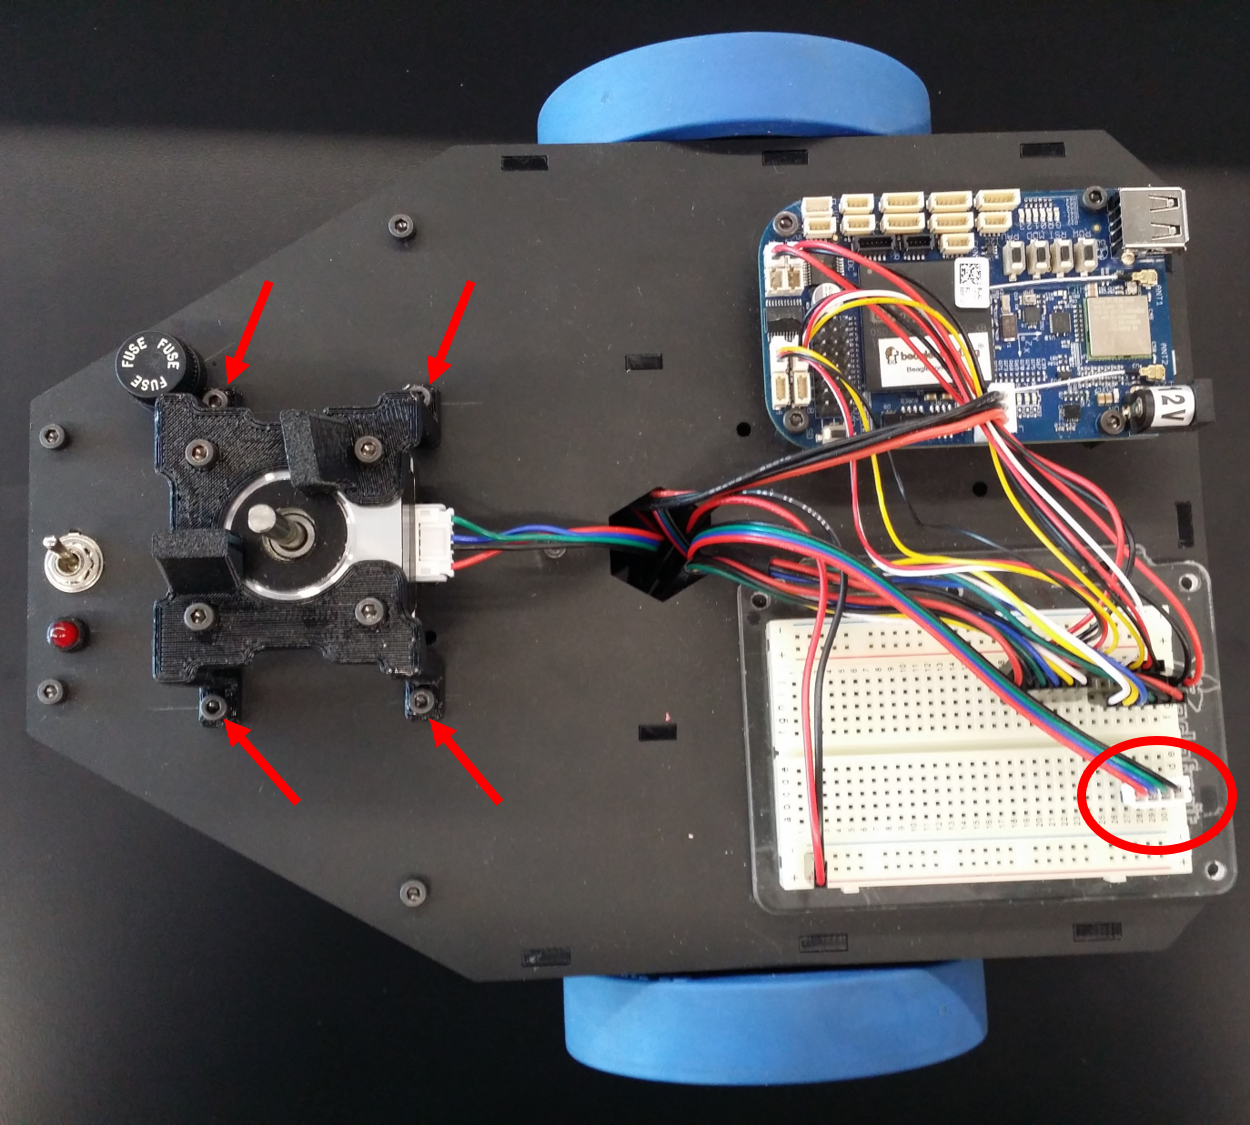
\includegraphics[width=3.7in]{figs/img/assembly/06-stepperMounting.png}
        \caption{Mounting Stepper Motor onto Budget Bot}
        \label{fig:stepperMounting}
    \end{figure}

    \item Using two 2-pin JST-ZH connectors, connect motor output channels 3 and 4 to the stepper motor windings (Fig. \ref{fig:stepperWiring}).
    \begin{figure}[H]
        \centering
        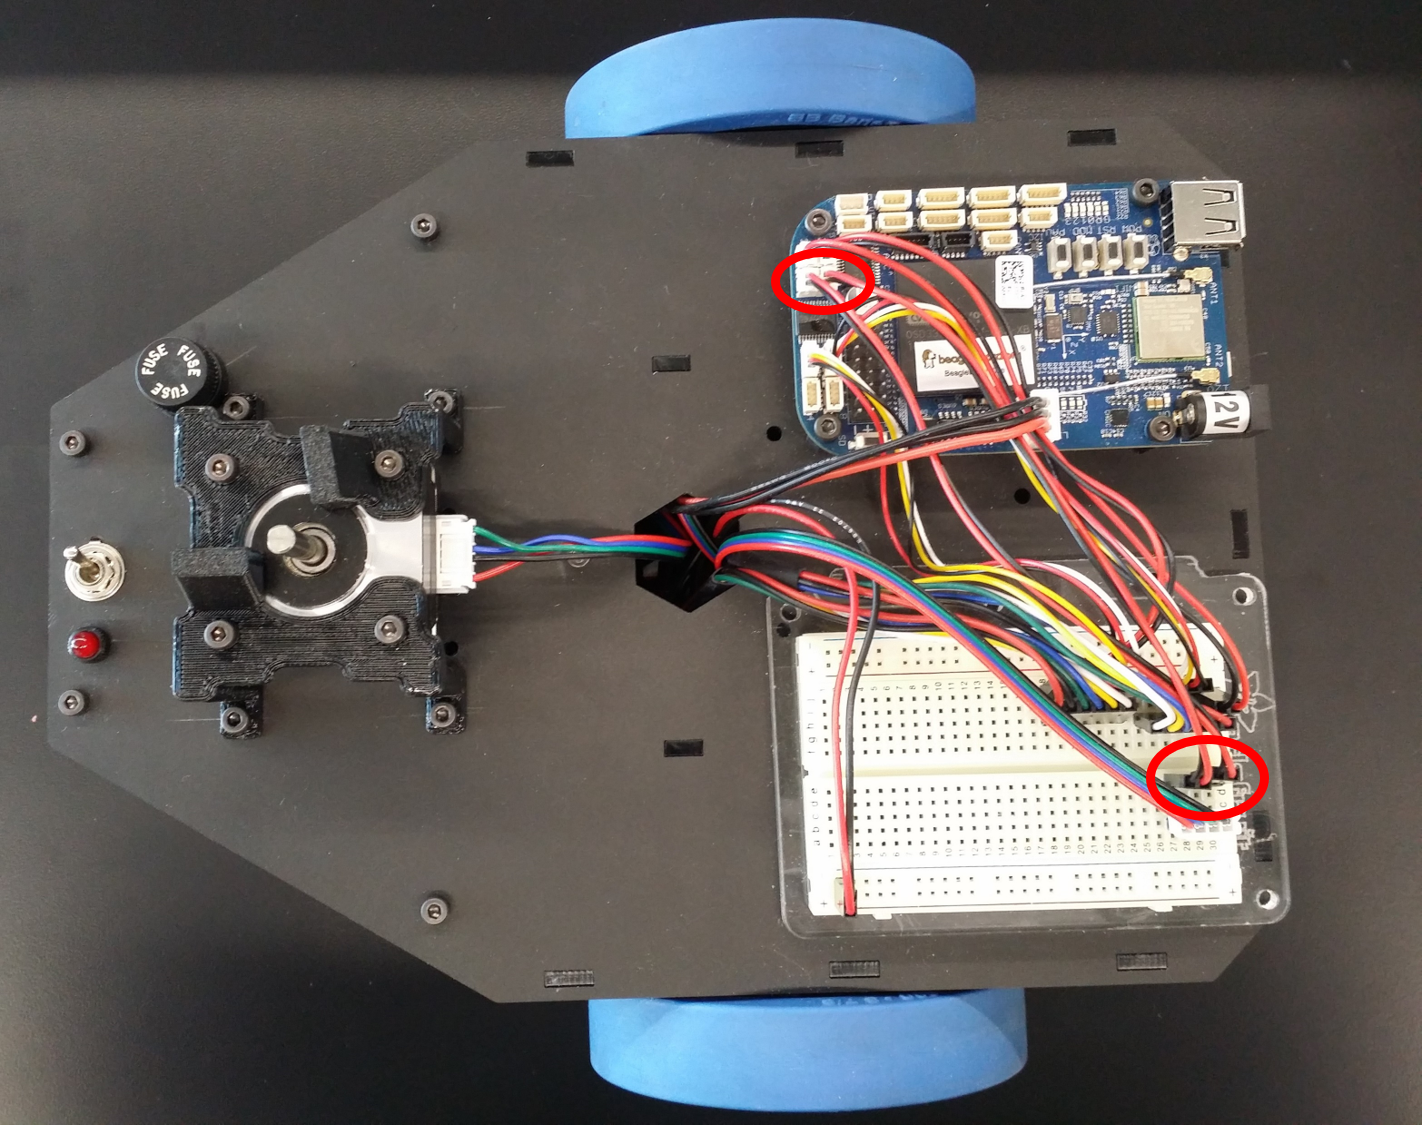
\includegraphics[width=4in]{figs/img/assembly/07-stepperWiring.png}
        \caption{Stepper Motor Wiring}
        \label{fig:stepperWiring}
    \end{figure}
    \pagebreak

    \item Insert a DG409DJ+ multiplexer across the center of the breadboard (Fig. \ref{fig:multiplexer}). Make sure the divot is toward the end of the breadboard to prevent mistakes during the rest of the assembly.
    \begin{figure}[H]
        \centering
        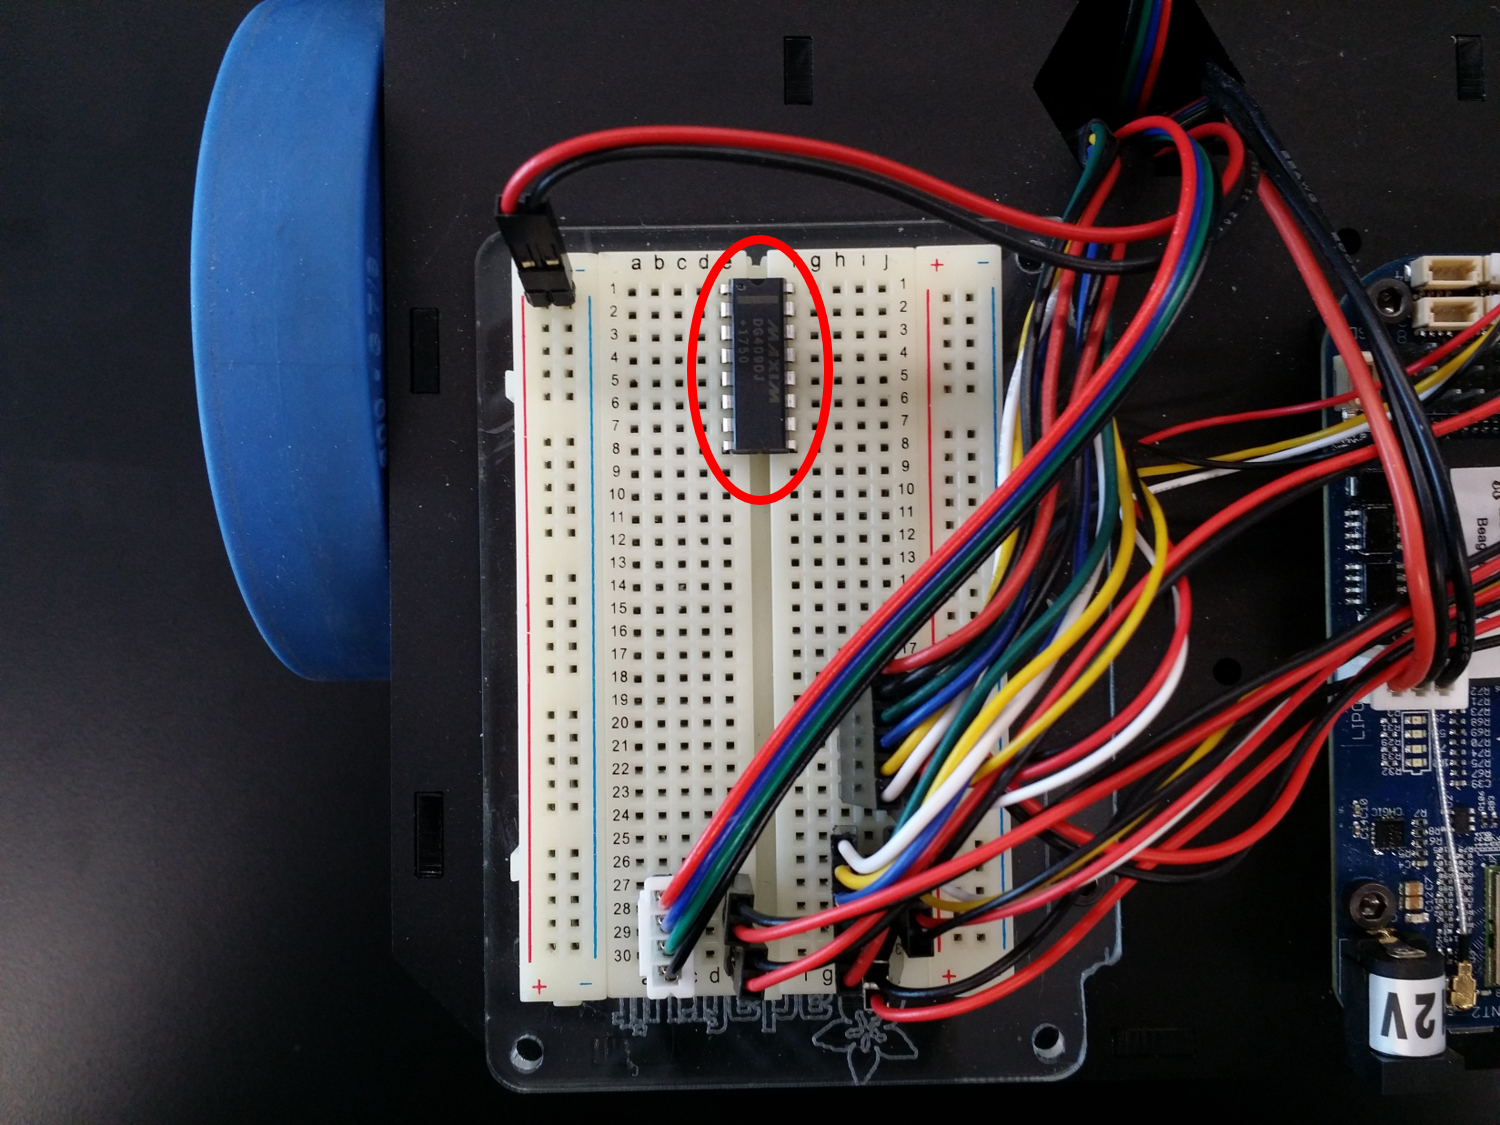
\includegraphics[width=4.2in]{figs/img/assembly/08-multiplexer.png}
        \caption{Multiplexer Installation}
        \label{fig:multiplexer}
    \end{figure}

    \item Connect battery power to the multiplexer by connecting V+ to pin 14 and GND to pin 15 of the multiplexer (Fig. \ref{fig:multiplexerPower}).
    \begin{figure}[H]
        \centering
        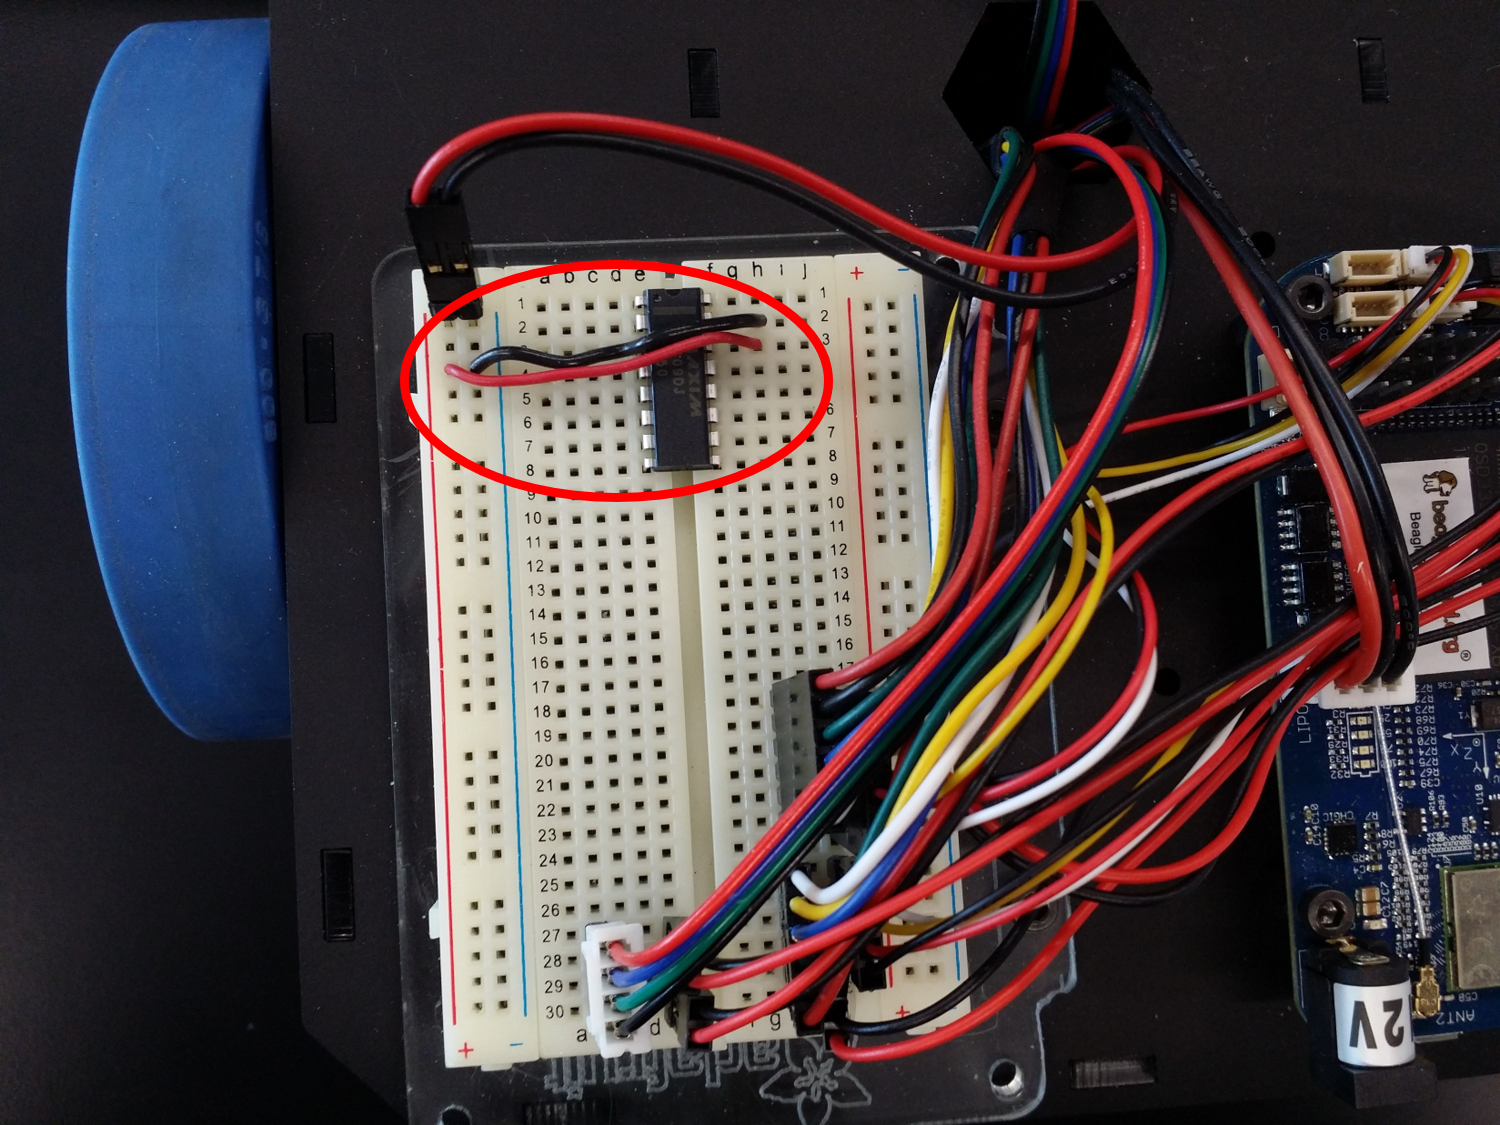
\includegraphics[width=4.2in]{figs/img/assembly/09-multiplexerPower.png}
        \caption{Powering the Multiplexer}
        \label{fig:multiplexerPower}
    \end{figure}
    \pagebreak

    \item Insert an LM1117 3.3V regulator into the breadboard. Place a 10\textmu F capacitor between the output terminal and ground. Connect the ground terminal to the battery ground and the input power terminal to the battery V+ (Fig. \ref{fig:regulator})
    \begin{figure}[H]
        \centering
        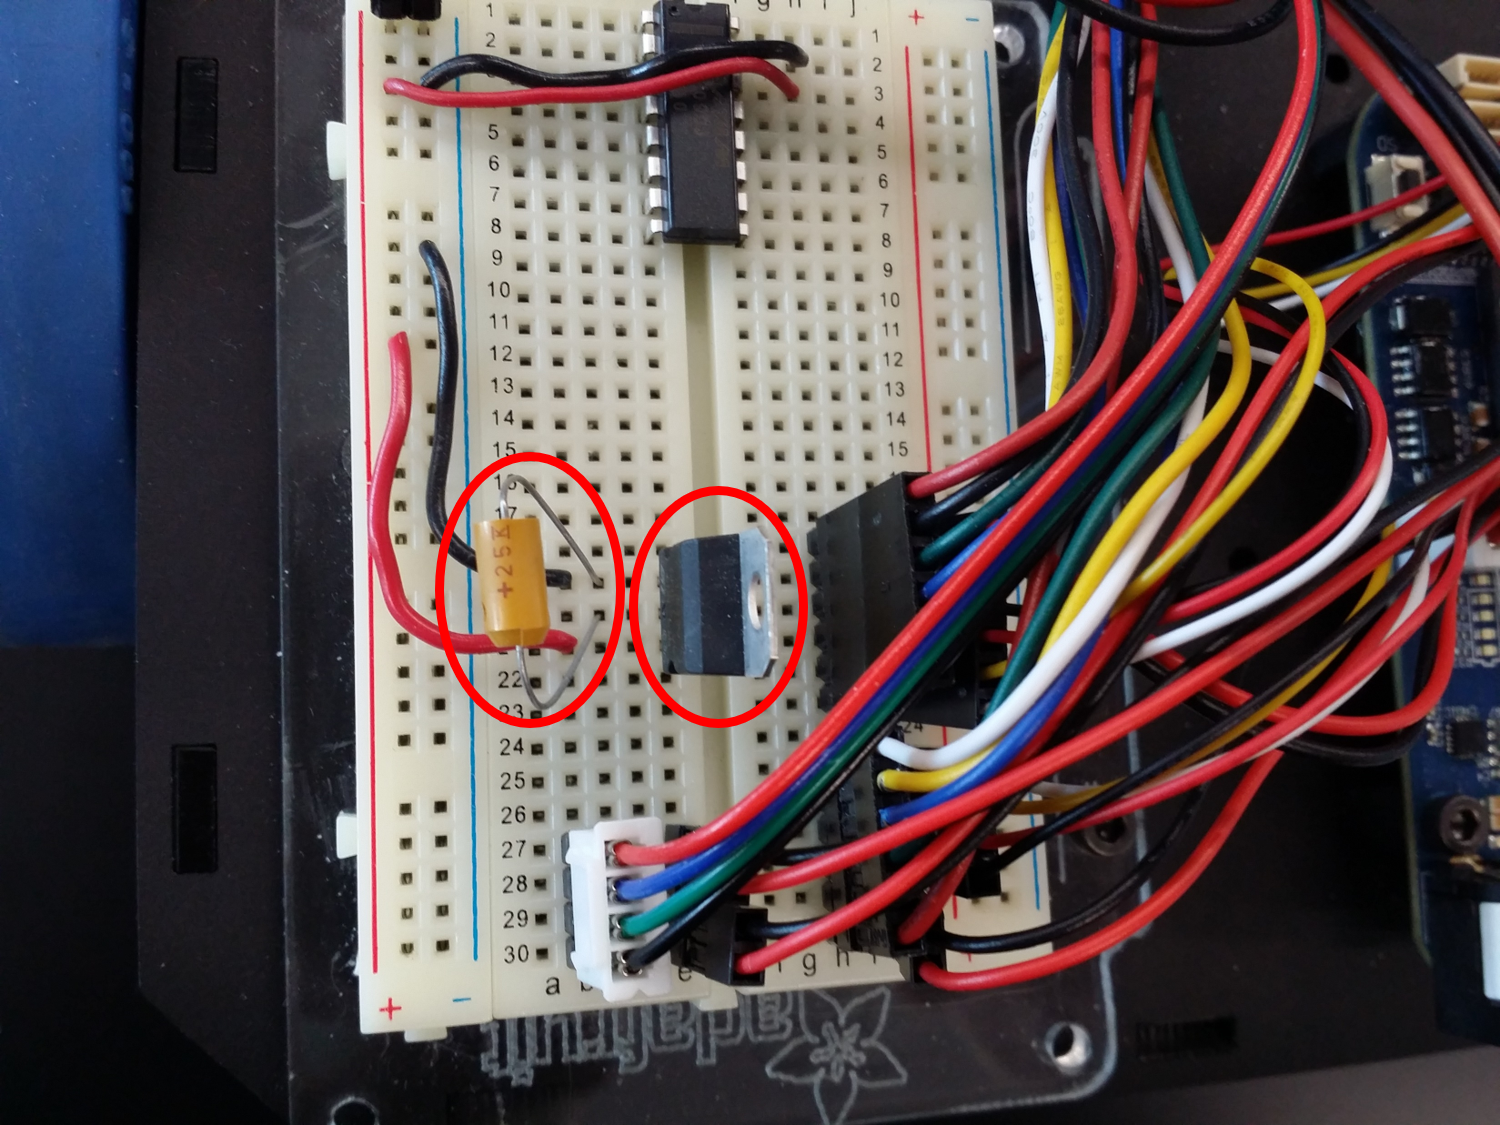
\includegraphics[width=3.8in]{figs/img/assembly/10-regulatorWiring.png}
        \caption{Regulator Installation}
        \label{fig:regulator}
    \end{figure}

    \item Connect +3.3V from GPIO1 to pin 2 on the multiplexer (Fig. \ref{fig:multiplexerWiring}, red arrows). Connect GPIO1 pins 1 and 2 to multiplexer pins 1 and 16, respectively (Fig. \ref{fig:multiplexerWiring}, green and orange arrows). Connect UART1 TX and RX to multiplexer pins 8 and 9, respectively (Fig. \ref{fig:multiplexerWiring}, yellow and purple arrows). Finally, connect UART5 TX and RX into the breadboard (Fig. \ref{fig:multiplexerWiring}, blue arrows).
    \begin{figure}[H]
        \centering
        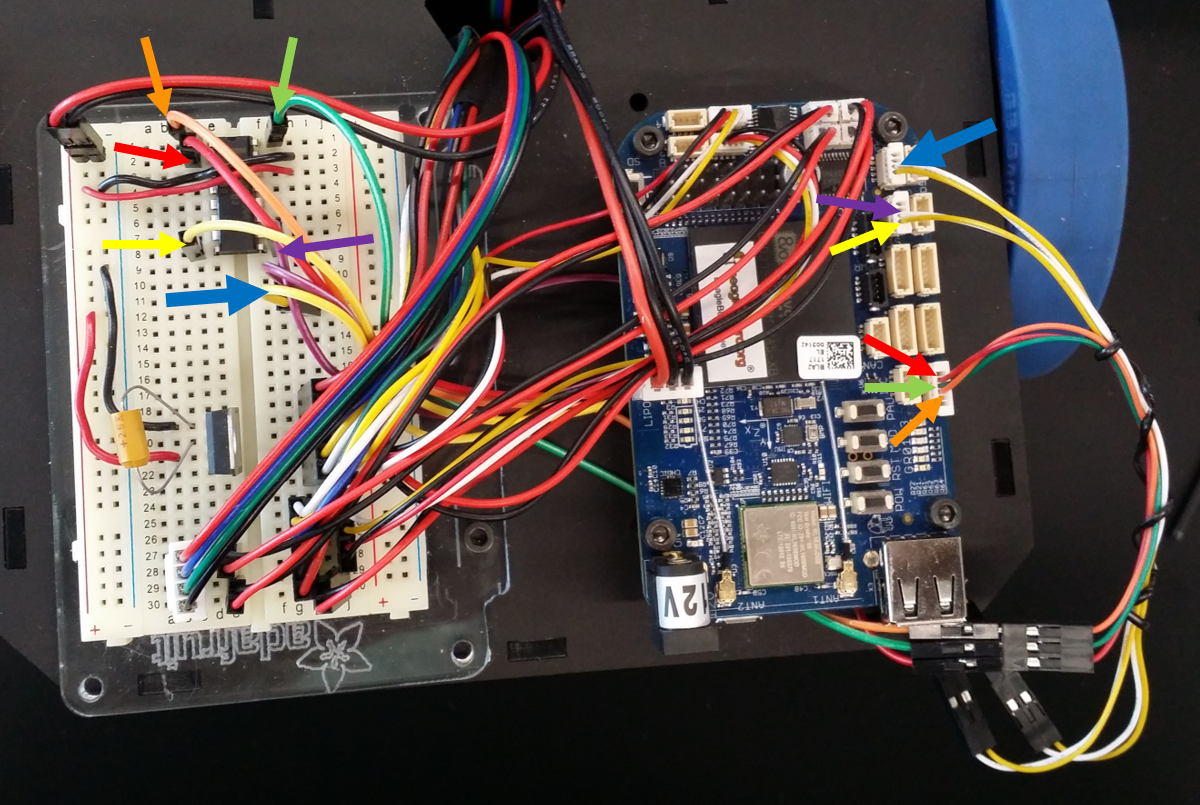
\includegraphics[width=4.8in]{figs/img/assembly/11-multiplexerBBBlueWiring.png}
        \caption{Connecting the Multiplexer to the BBBlue}
        \label{fig:multiplexerWiring}
    \end{figure}
    \pagebreak

    \item Prepare the reflector dishes, top plate, and bottom frame. Also prepare some 8mm and 10mm M3 screws and some M3 nuts (Fig. \ref{fig:reflectorParts}).
    \begin{figure}[H]
        \centering
        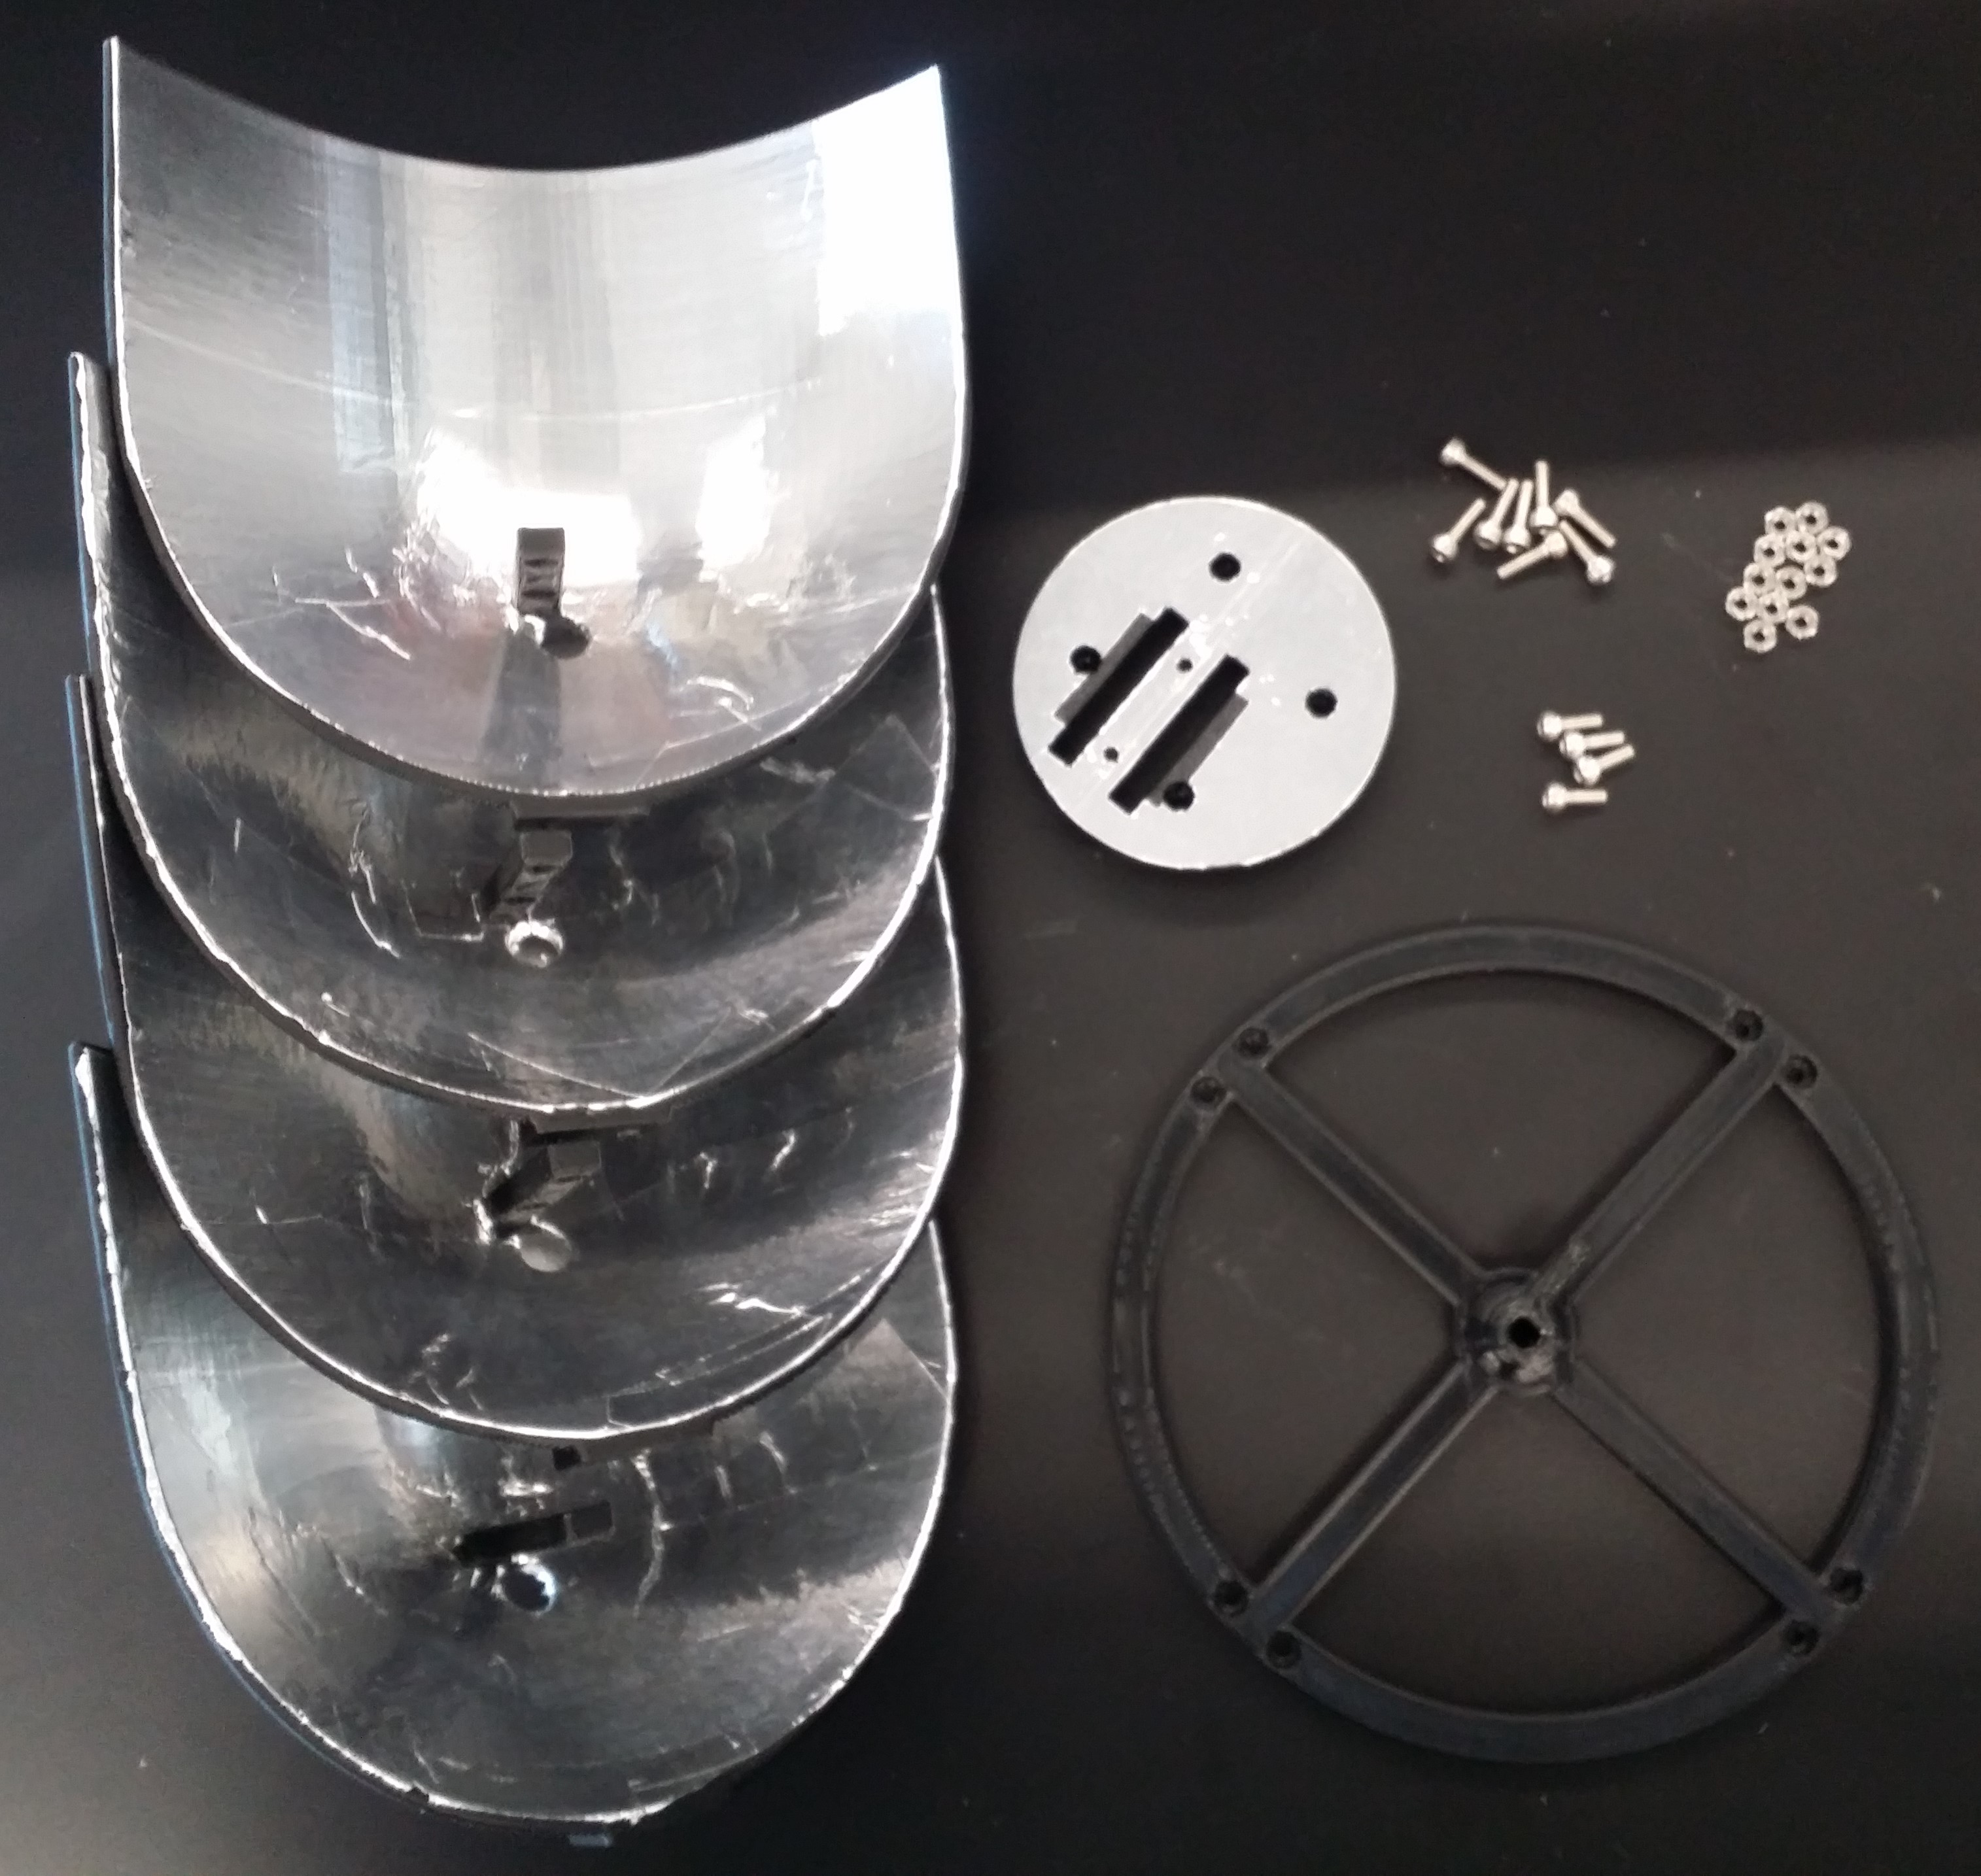
\includegraphics[width=4.4in]{figs/img/assembly/12-reflectorParts.jpg}
        \caption{Reflector Parts}
        \label{fig:reflectorParts}
    \end{figure}

    \item Insert an M3 nut into the slot at the top of one of the reflector dishes (Fig. \ref{fig:reflectorTopNut}).
    \begin{figure}[H]
        \centering
        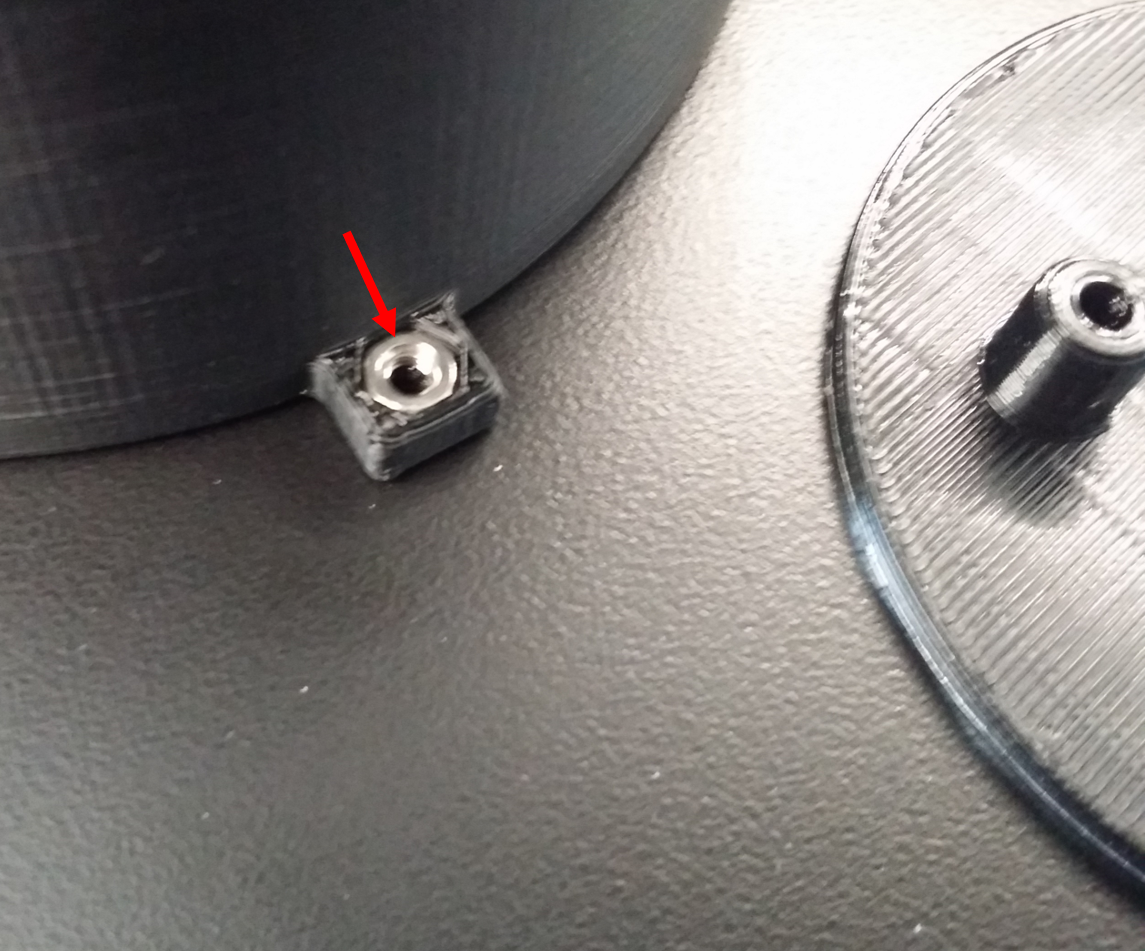
\includegraphics[width=3.6in]{figs/img/assembly/13-reflectorTopNut.png}
        \caption{Top Reflector Nut}
        \label{fig:reflectorTopNut}
    \end{figure}
    \pagebreak

    \item Attach the top plate using an 8mm M3 screw (Fig. \ref{fig:reflectorTopPlate}).
    \begin{figure}[H]
        \centering
        \includegraphics[width=4.1in]{figs/img/assembly/14-reflectorTopPlate.jpg}
        \caption{Attaching Top Plate}
        \label{fig:reflectorTopPlate}
    \end{figure}

    \item Repeat steps 13 and 14 to attach all of the reflector dishes to the top plate (Fig. \ref{fig:finishedTopPlate}).
    \begin{figure}[H]
        \centering
        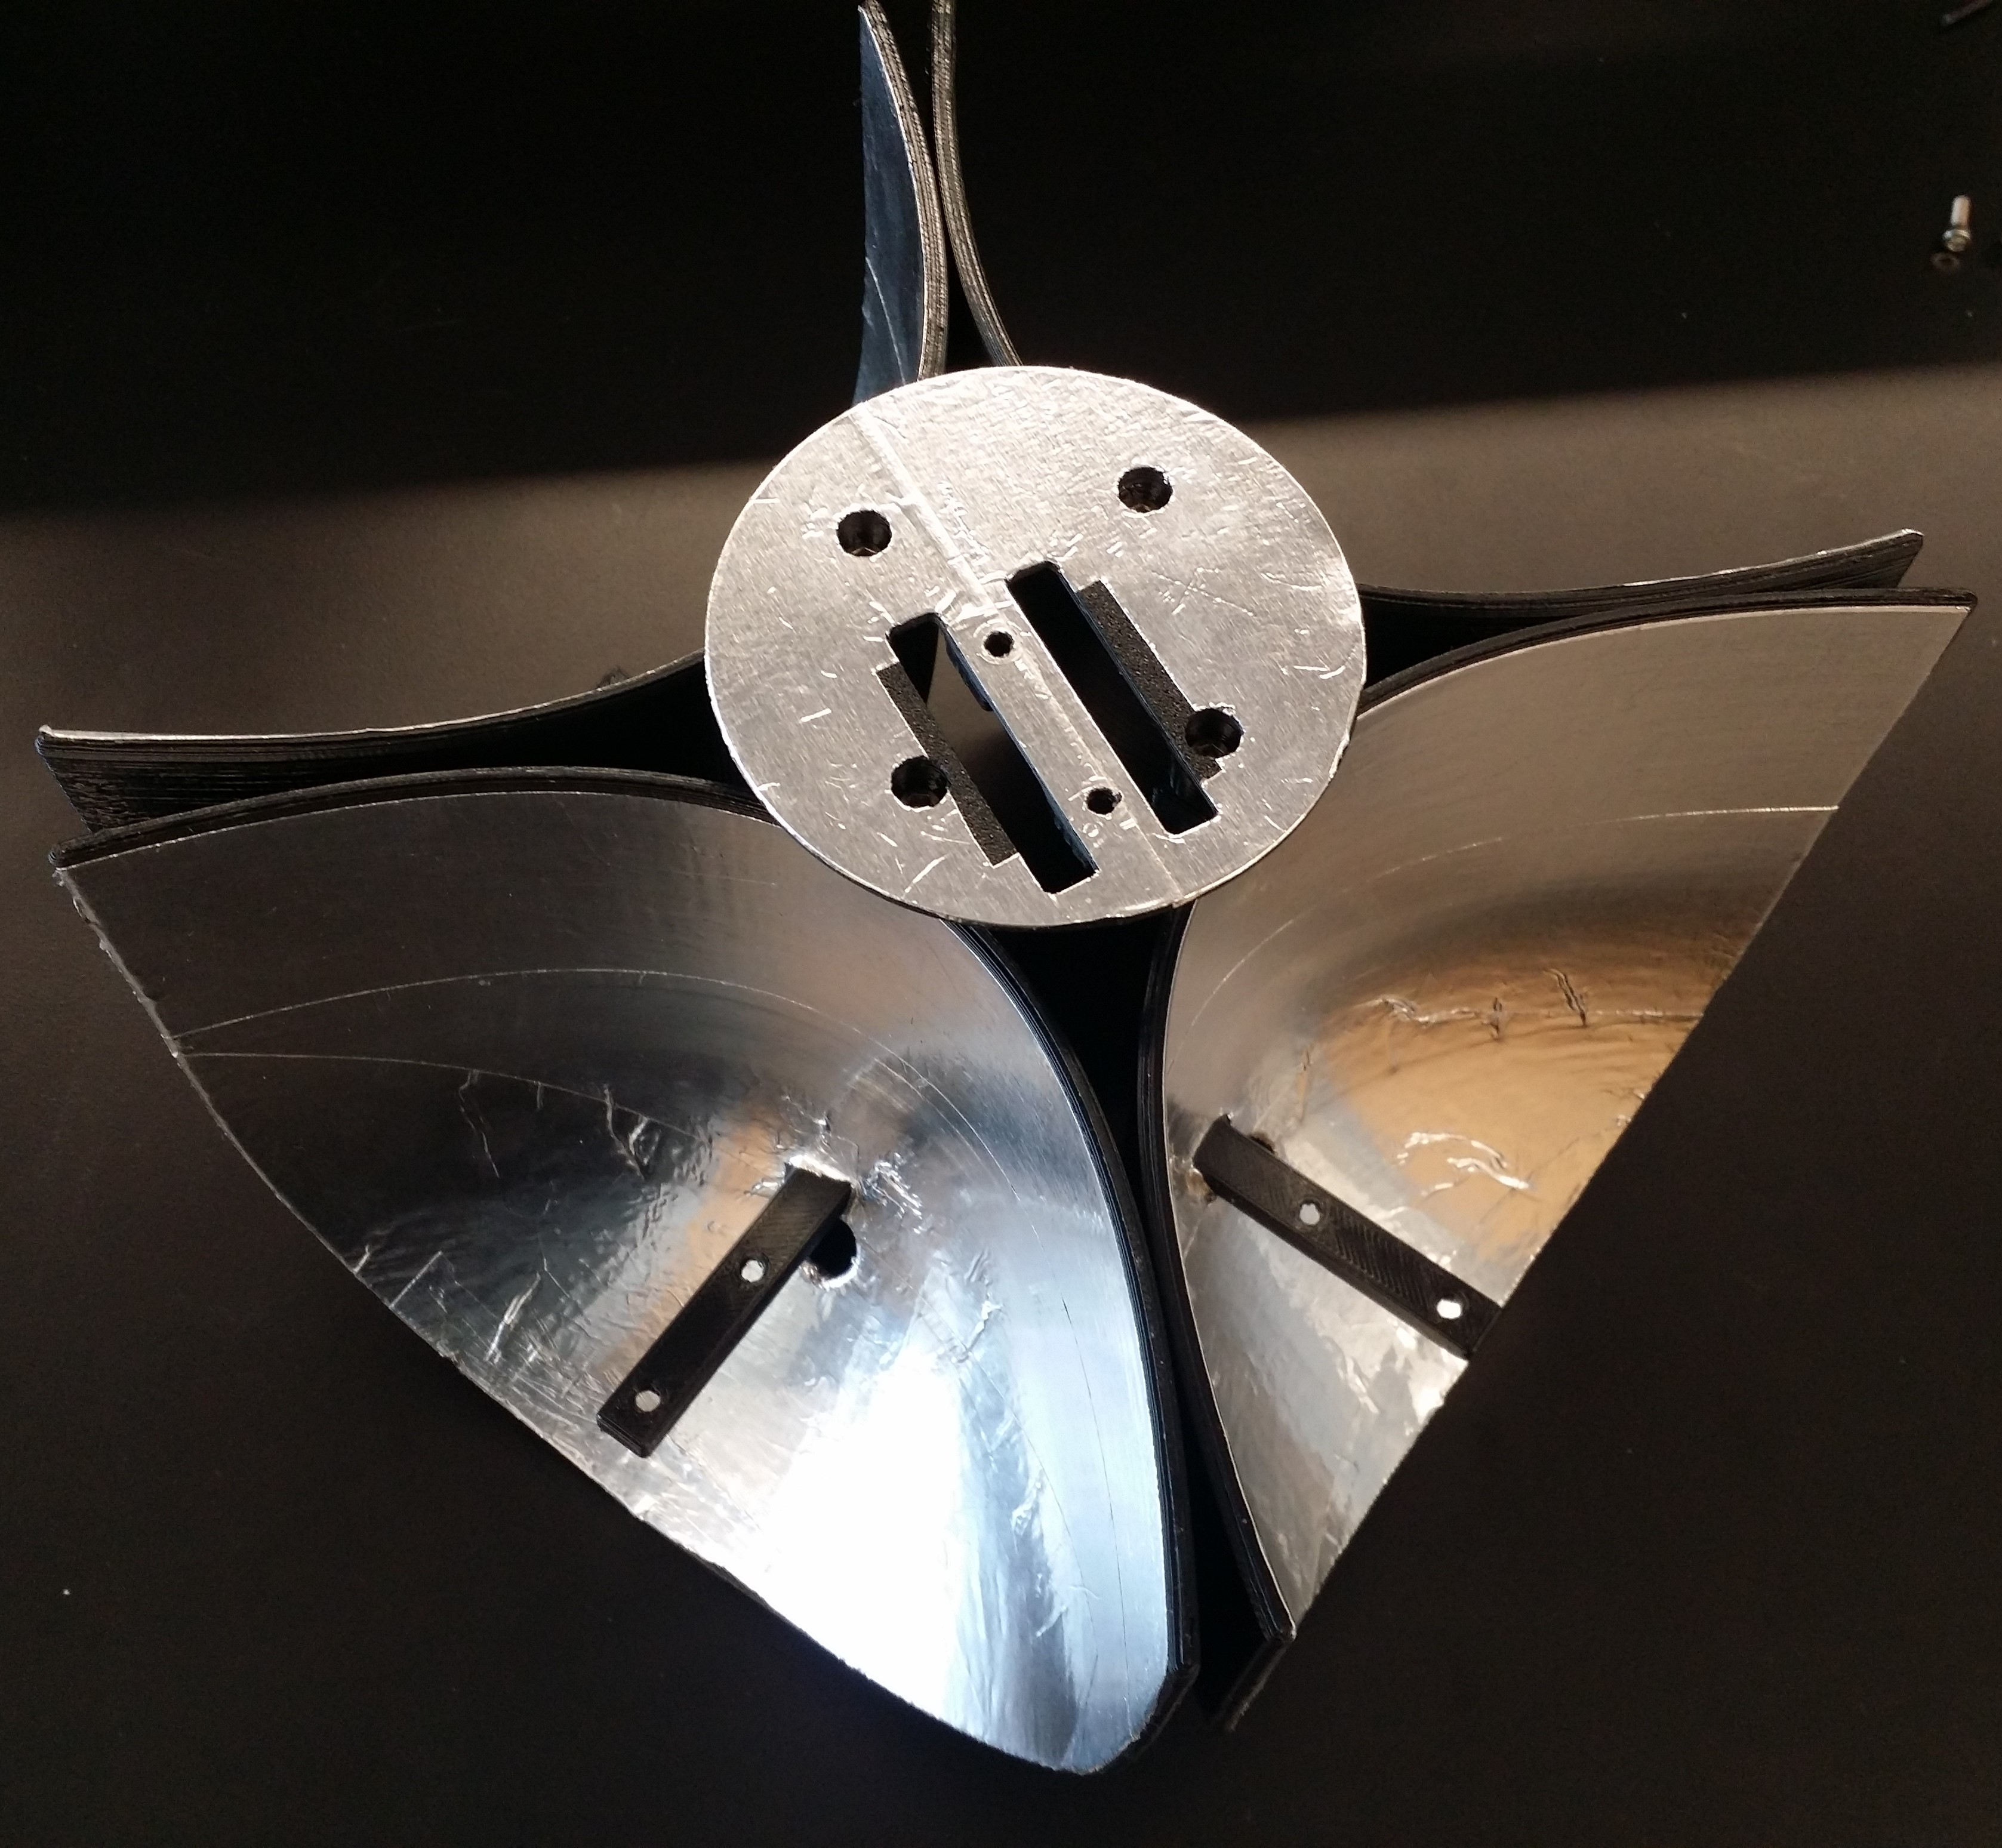
\includegraphics[width=4.1in]{figs/img/assembly/15-finishedReflectorTopPlate.jpg}
        \caption{Finished Top Plate}
        \label{fig:finishedTopPlate}
    \end{figure}
    \pagebreak

    \item Insert wires from the bottom of the reflectors up through the left slot (when viewed from above) and connect them to the VCC (red), DOUT (purple), DIN (yellow), and VSS (black) pins of an XBee adapter board (Fig. \ref{fig:topXBeeWiring}).
    \begin{figure}[H]
        \centering
        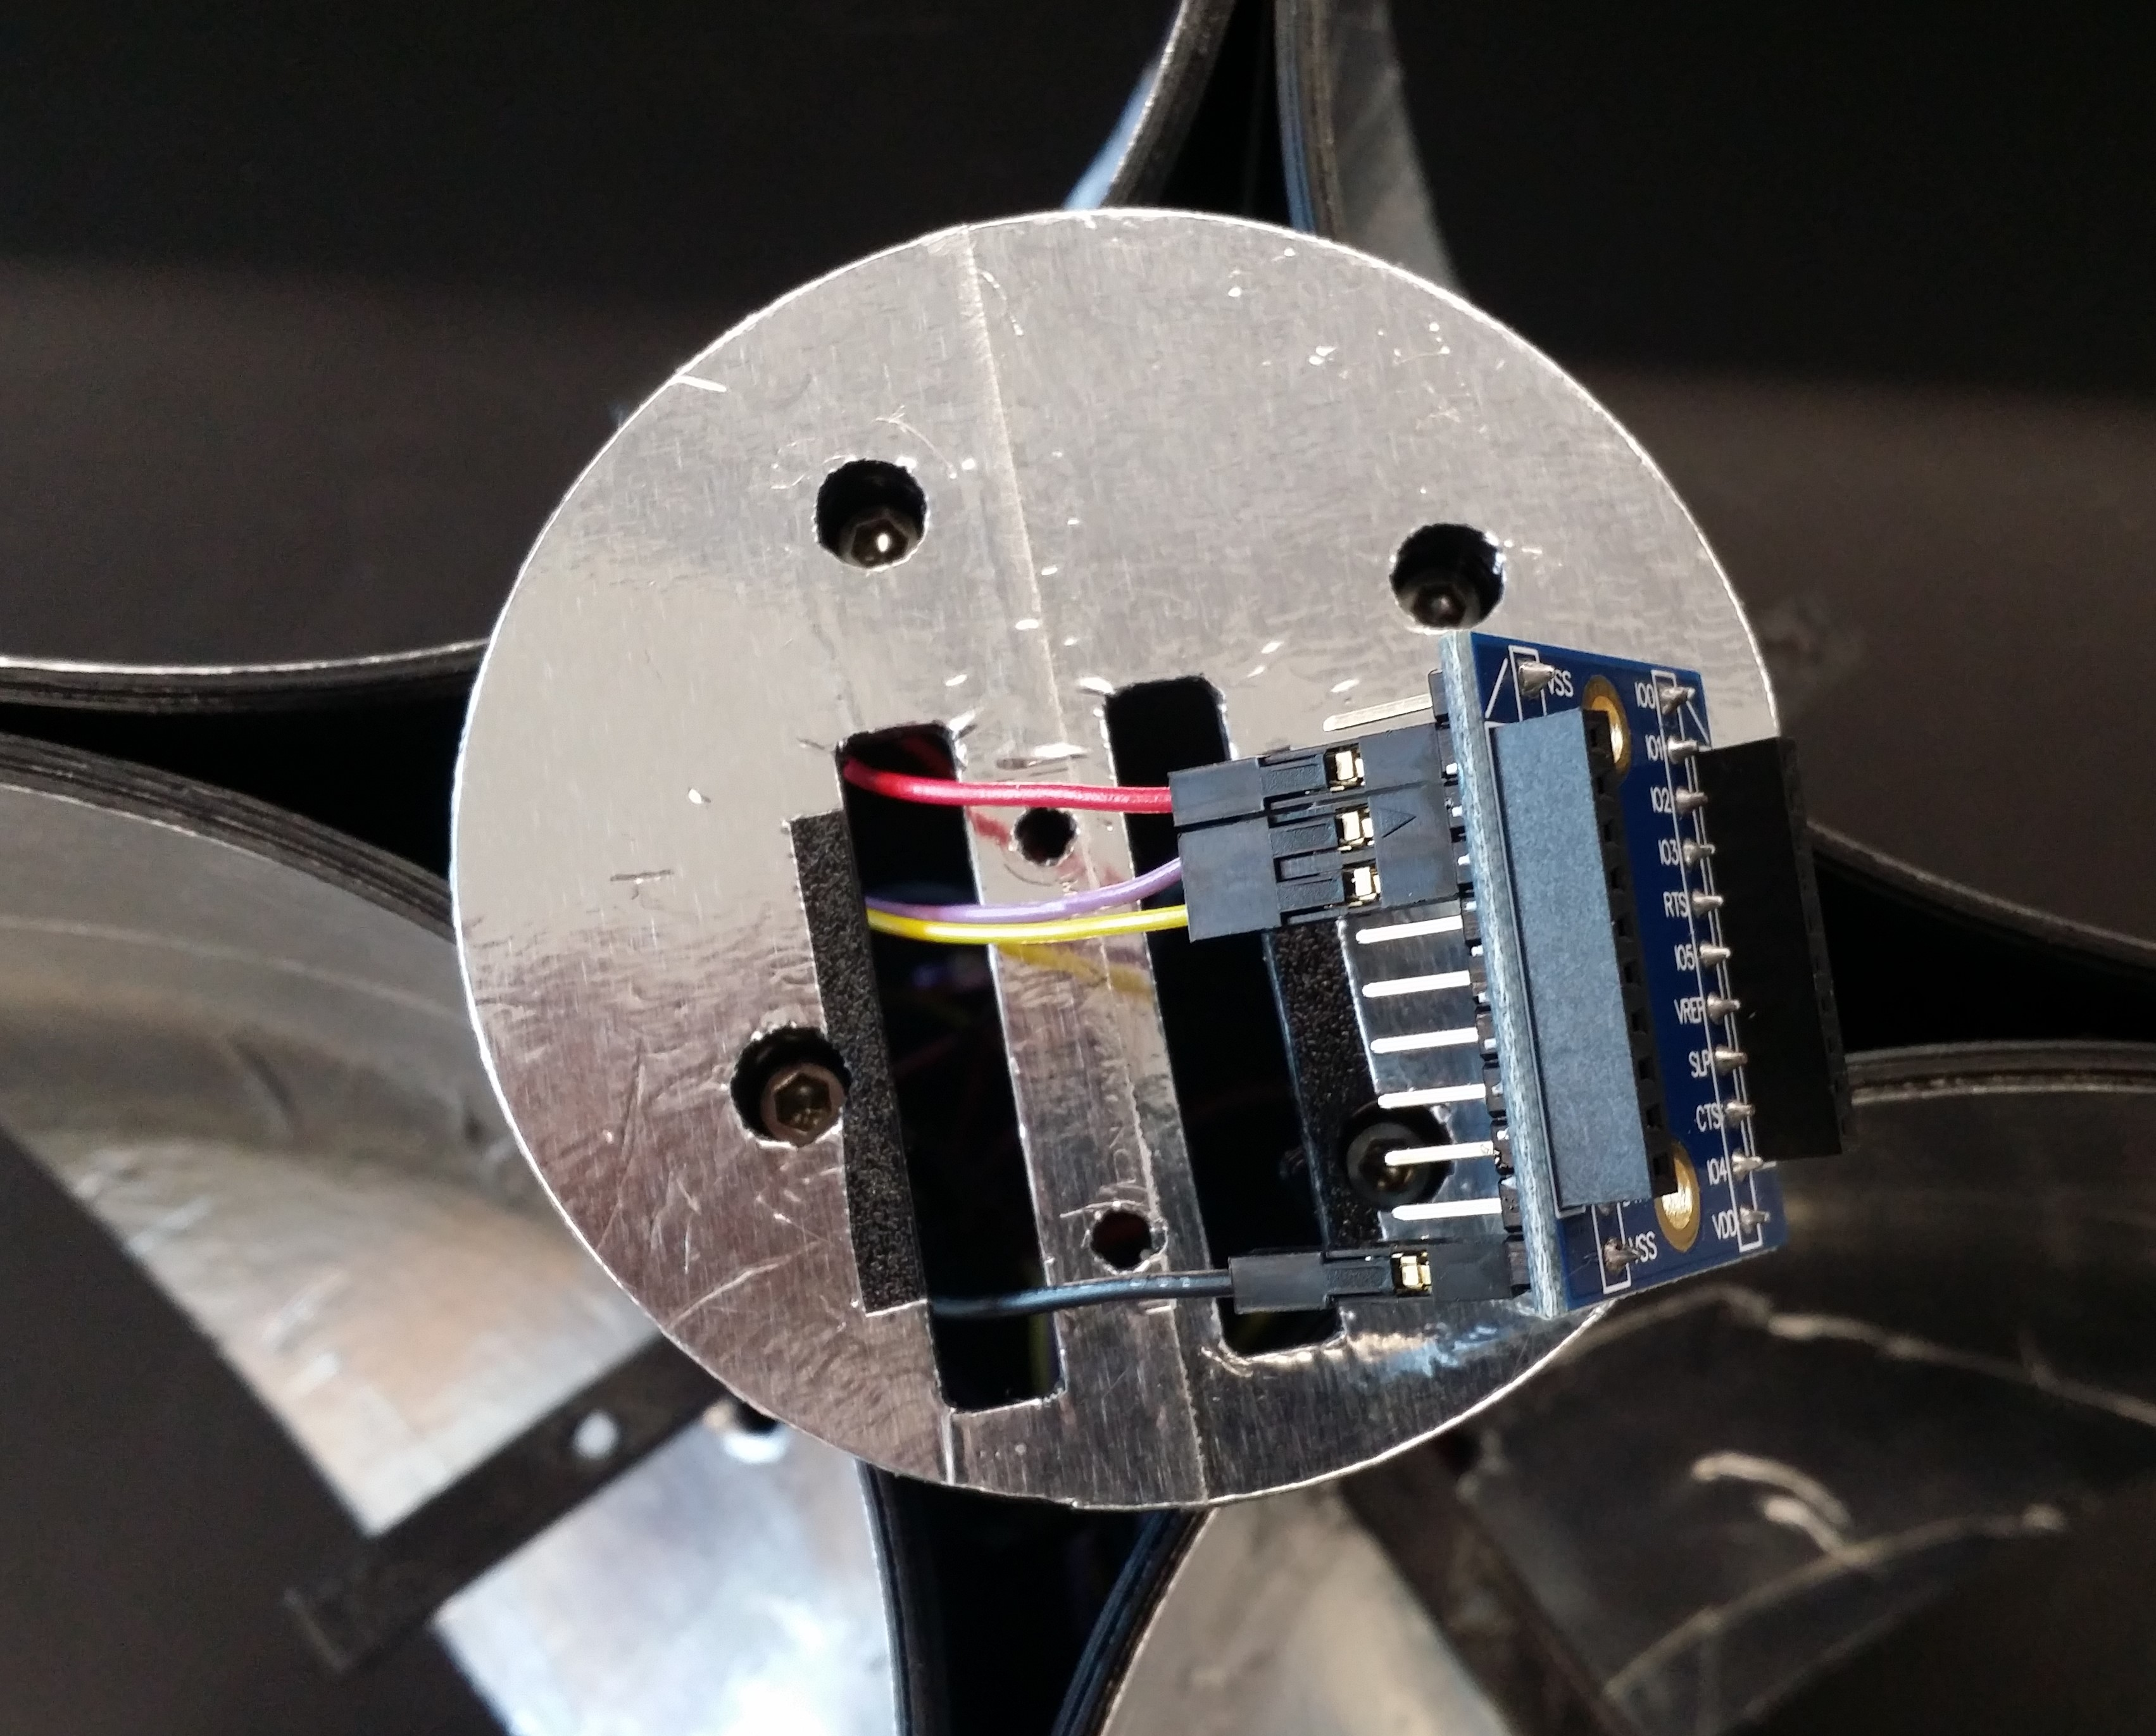
\includegraphics[width=4.2in]{figs/img/assembly/16-topXBeeWiring.jpg}
        \caption{Wiring for Top XBee}
        \label{fig:topXBeeWiring}
    \end{figure}

    \item Insert two M3 nuts into the slots on the underside of the top plate (Fig. \ref{fig:topXBeeNuts}).
    \begin{figure}[H]
        \centering
        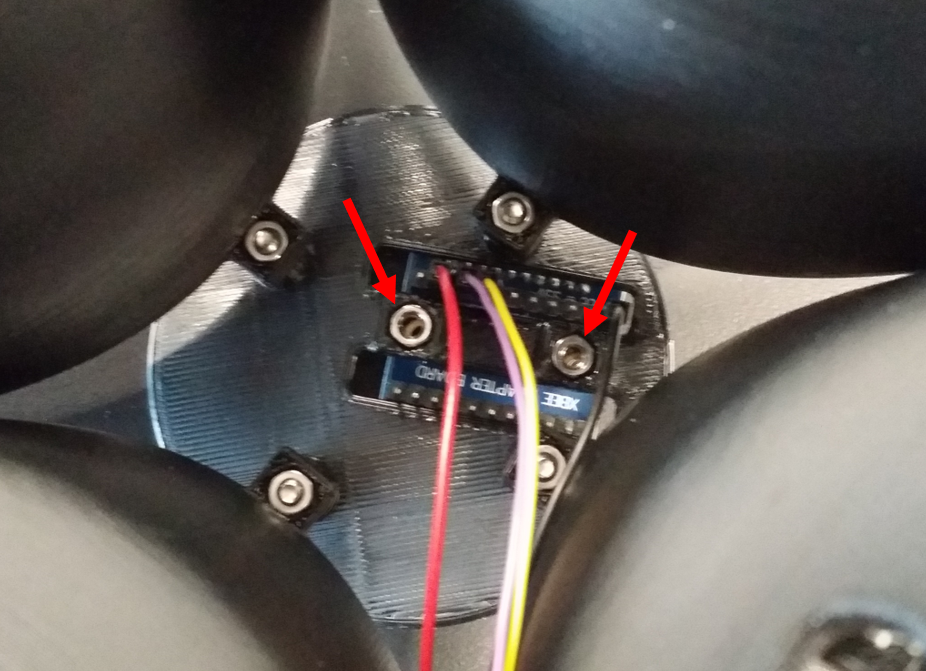
\includegraphics[width=4.2in]{figs/img/assembly/17-topXBeeNuts.png}
        \caption{Nuts for top XBee}
        \label{fig:topXBeeNuts}
    \end{figure}
    \pagebreak

    \item Attach the XBee adapter board to the top plate using two 8mm M3 screws (Fig. \ref{fig:topXBeeMounting}).
    \begin{figure}[H]
        \centering
        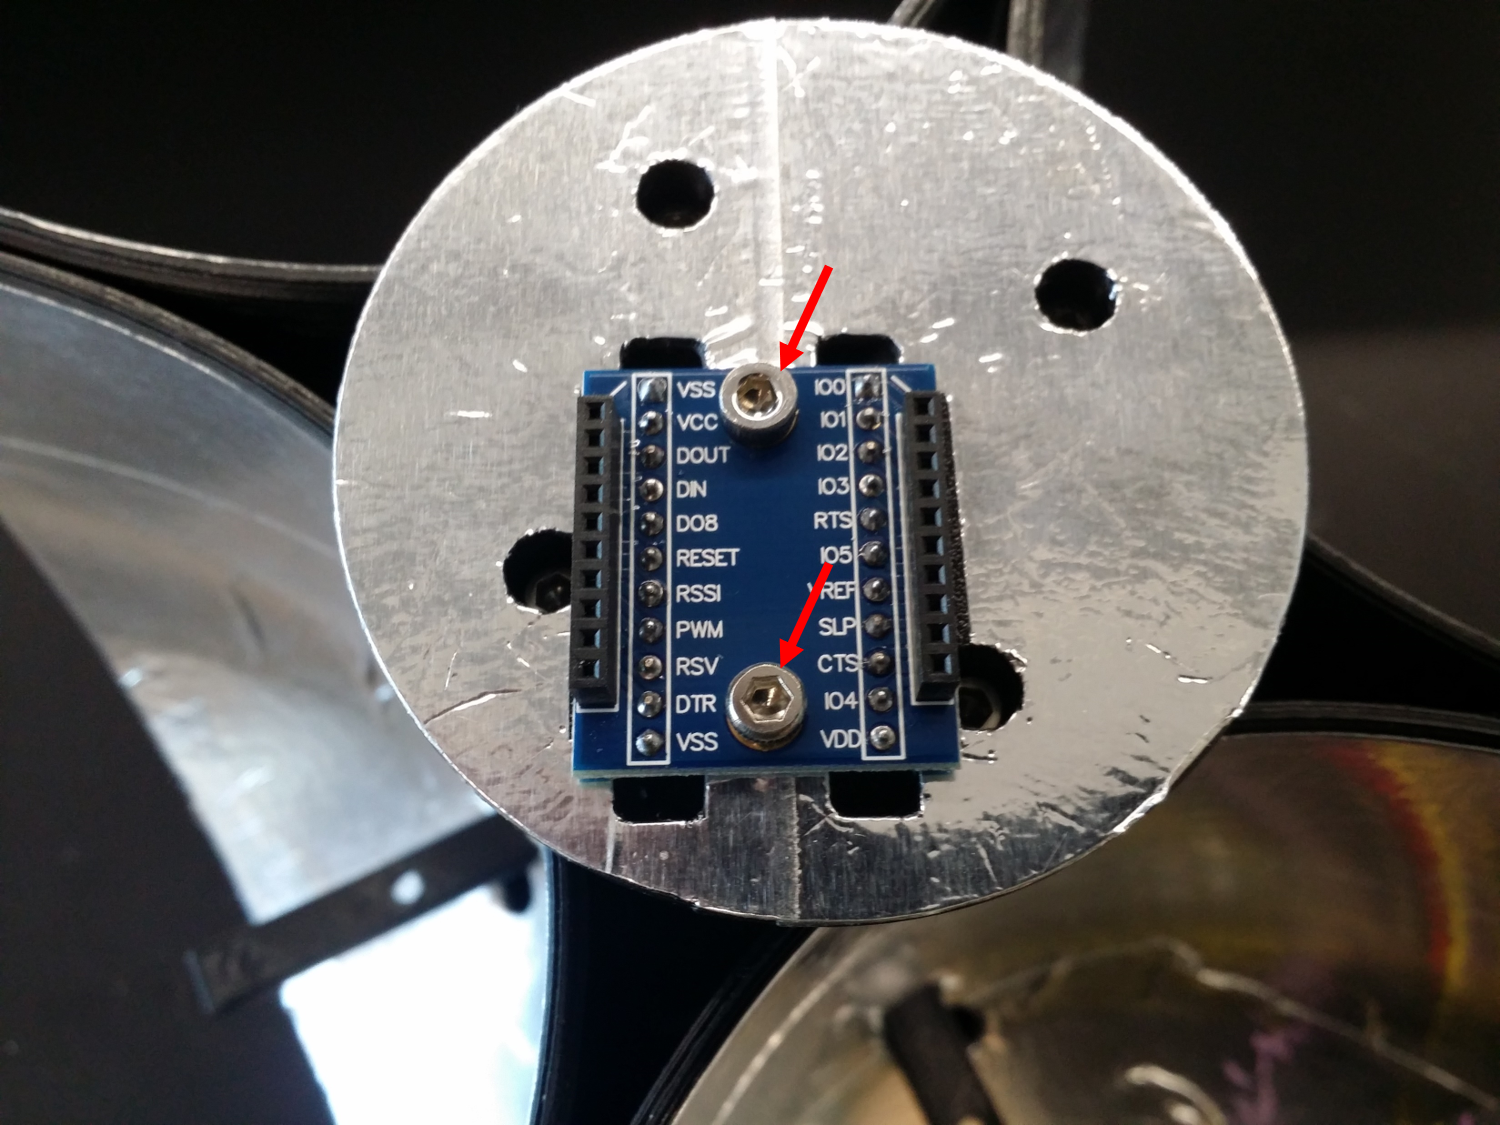
\includegraphics[width=4.2in]{figs/img/assembly/18-topXBeeMounting.png}
        \caption{Mounting the Top XBee}
        \label{fig:topXBeeMounting}
    \end{figure}

    \item Insert wires through the back of a reflector dish and connect them to the VCC (red), DOUT (purple), DIN (yellow), and VSS (black) pins of an XBee adapter board (Fig. \ref{fig:sideXBeeWiring}). It is useful to number the purple and yellow wires at both ends with the reflector number. The reflectors should be numbered 1 through 4 going clockwise.
    \begin{figure}[H]
        \centering
        \includegraphics[width=4.2in]{figs/img/assembly/19-sideXBeeWiring.jpg}
        \caption{Wiring a Side XBee}
        \label{fig:sideXBeeWiring}
    \end{figure}
    \pagebreak

    \item Insert two M3 nuts into the underside of the support protruding from the reflector (Fig. \ref{fig:sideXBeeNuts})
    \begin{figure}[H]
        \centering
        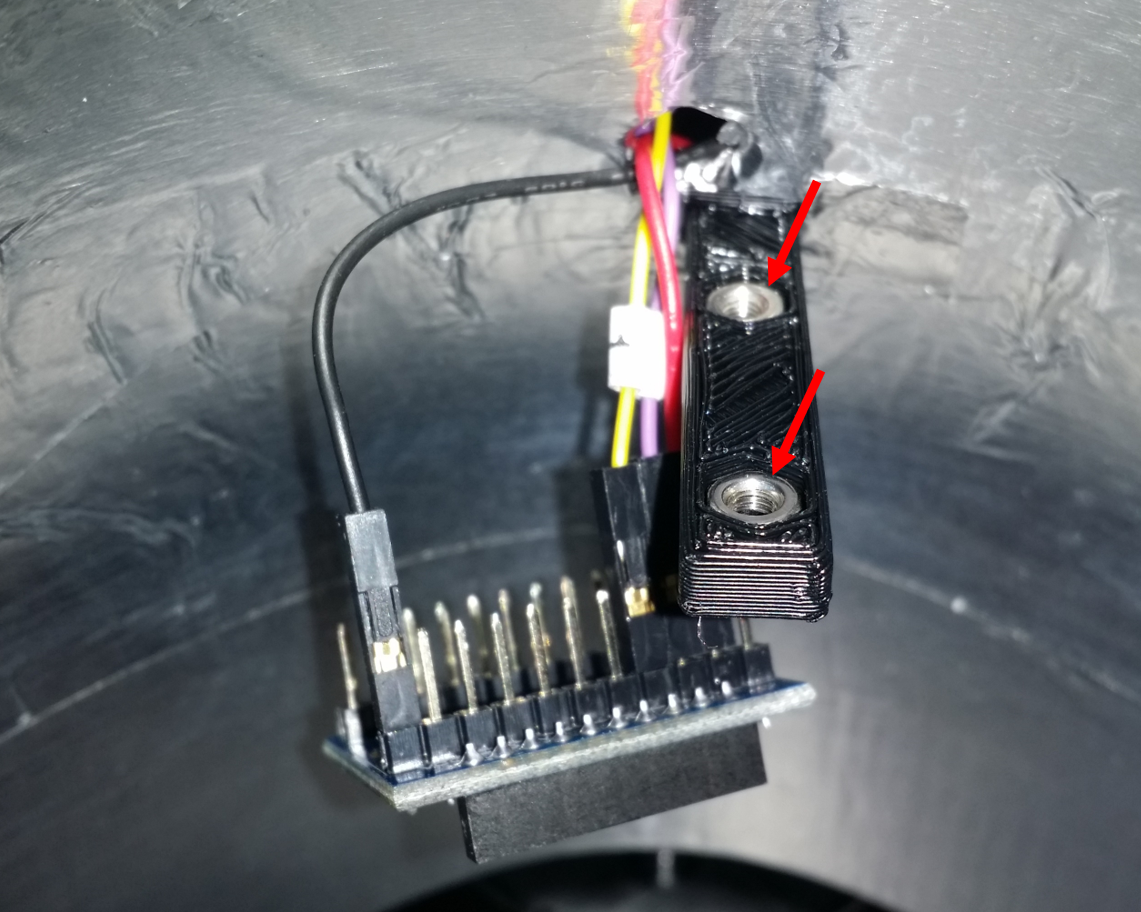
\includegraphics[width=4.2in]{figs/img/assembly/20-sideXBeeNuts.png}
        \caption{Nuts for Side XBee}
        \label{fig:sideXBeeNuts}
    \end{figure}

    \item Mount the XBee adapter board using two 8mm M3 screws (Fig. \ref{fig:sideXBeeMounting}). Make sure the board is oriented such that the antenna of the XBee will be toward the reflective surface.
    \begin{figure}[H]
        \centering
        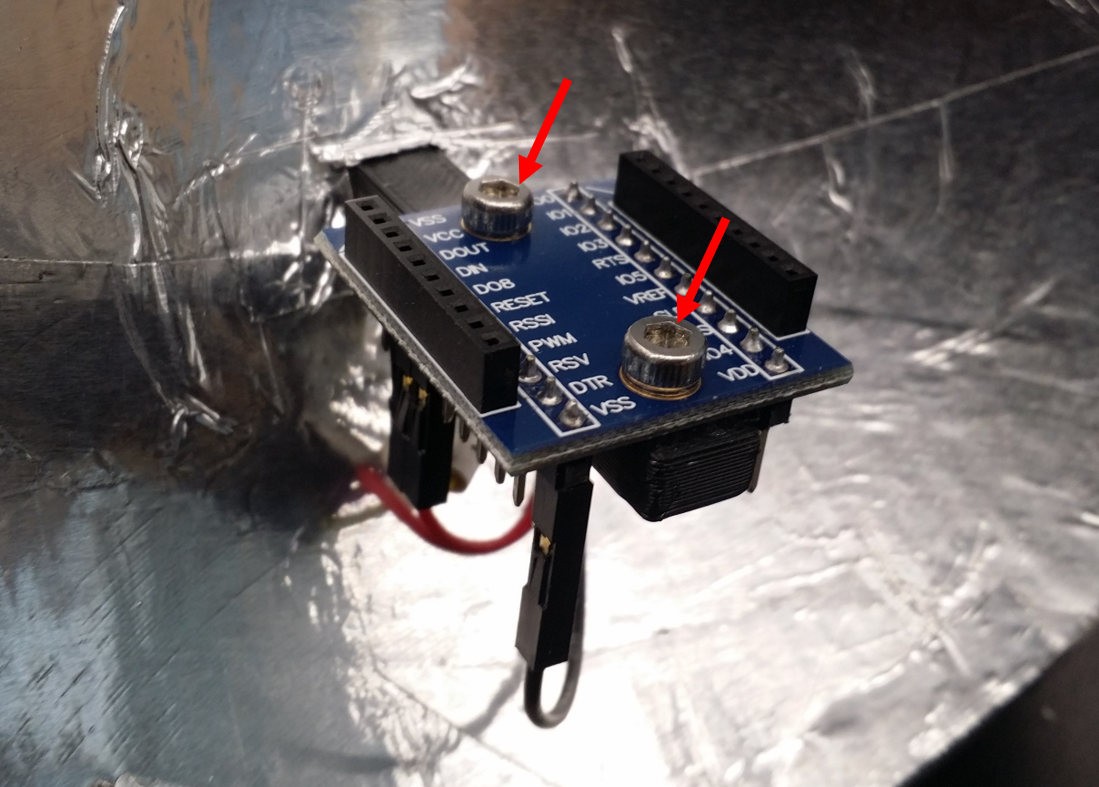
\includegraphics[width=4.2in]{figs/img/assembly/21-sideXBeeMounting.png}
        \caption{Mounting a Side XBee}
        \label{fig:sideXBeeMounting}
    \end{figure}
    \pagebreak

    \item Repeat steps 19 through 21 to mount XBee adapter boards into each of the four reflectors (Fig. \ref{fig:finishedSideXBees}).
    \begin{figure}[H]
        \centering
        \includegraphics[width=3.9in]{figs/img/assembly/22-finishedSideXBees.jpg}
        \caption{All Side XBees Mounted}
        \label{fig:finishedSideXBees}
    \end{figure}

    \item Wrap the wires coming from the reflector to keep them bundled into a single cable. Terminate the ends such that there is a 2-pin connector for +3.3V and GND (Fig. \ref{fig:reflectorWires}, red arrow), a 2-pin connector for the TX and RX to the top XBee (Fig. \ref{fig:reflectorWires}, blue arrow), a 4-pin connector for the TX pins of all four side XBees (Fig. \ref{fig:reflectorWires}, purple arrow), and a 4-pin connector for the RX pins of all four side XBees (Fig. \ref{fig:reflectorWires}, yellow arrow). Once again, it is useful to number both ends of the TX and RX wires to the side XBees.
    \begin{figure}[H]
        \centering
        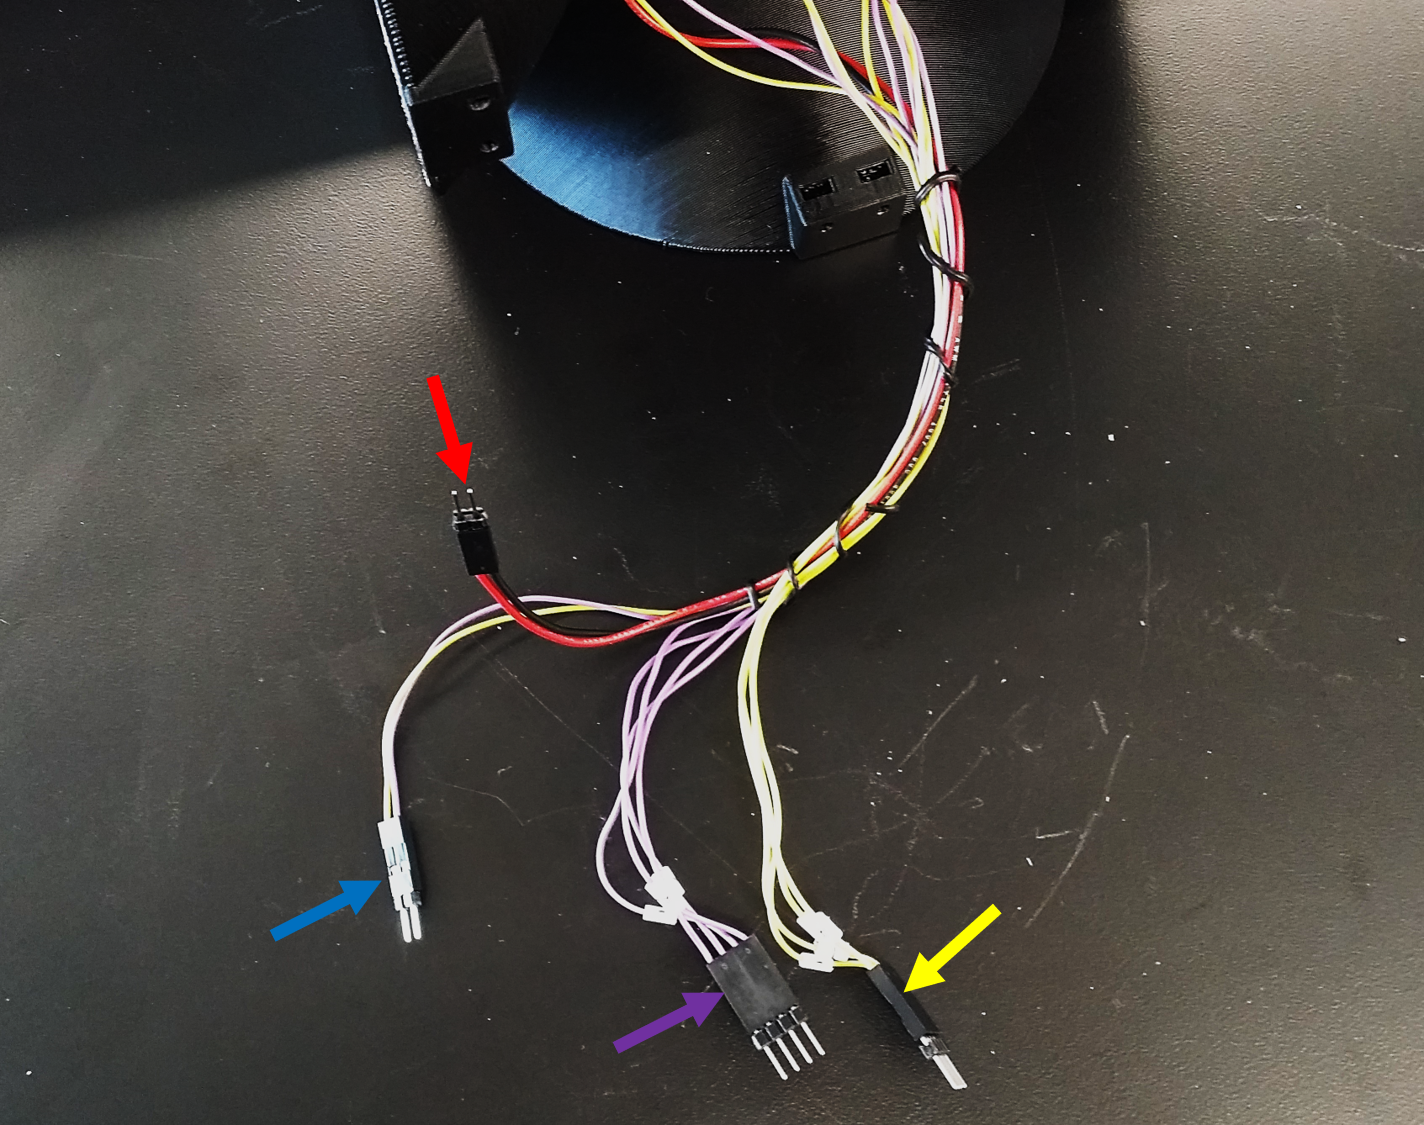
\includegraphics[width=3.9in]{figs/img/assembly/23-reflectorWireEnds.png}
        \caption{Reflector Wire Ends}
        \label{fig:reflectorWires}
    \end{figure}
    \pagebreak

    \item Insert two M3 nuts into the slots at the bottom of a reflector (Fig. \ref{fig:bottomNuts}). The nuts should recess into a hexagonal slot that prevents them from rotating.
    \begin{figure}[H]
        \centering
        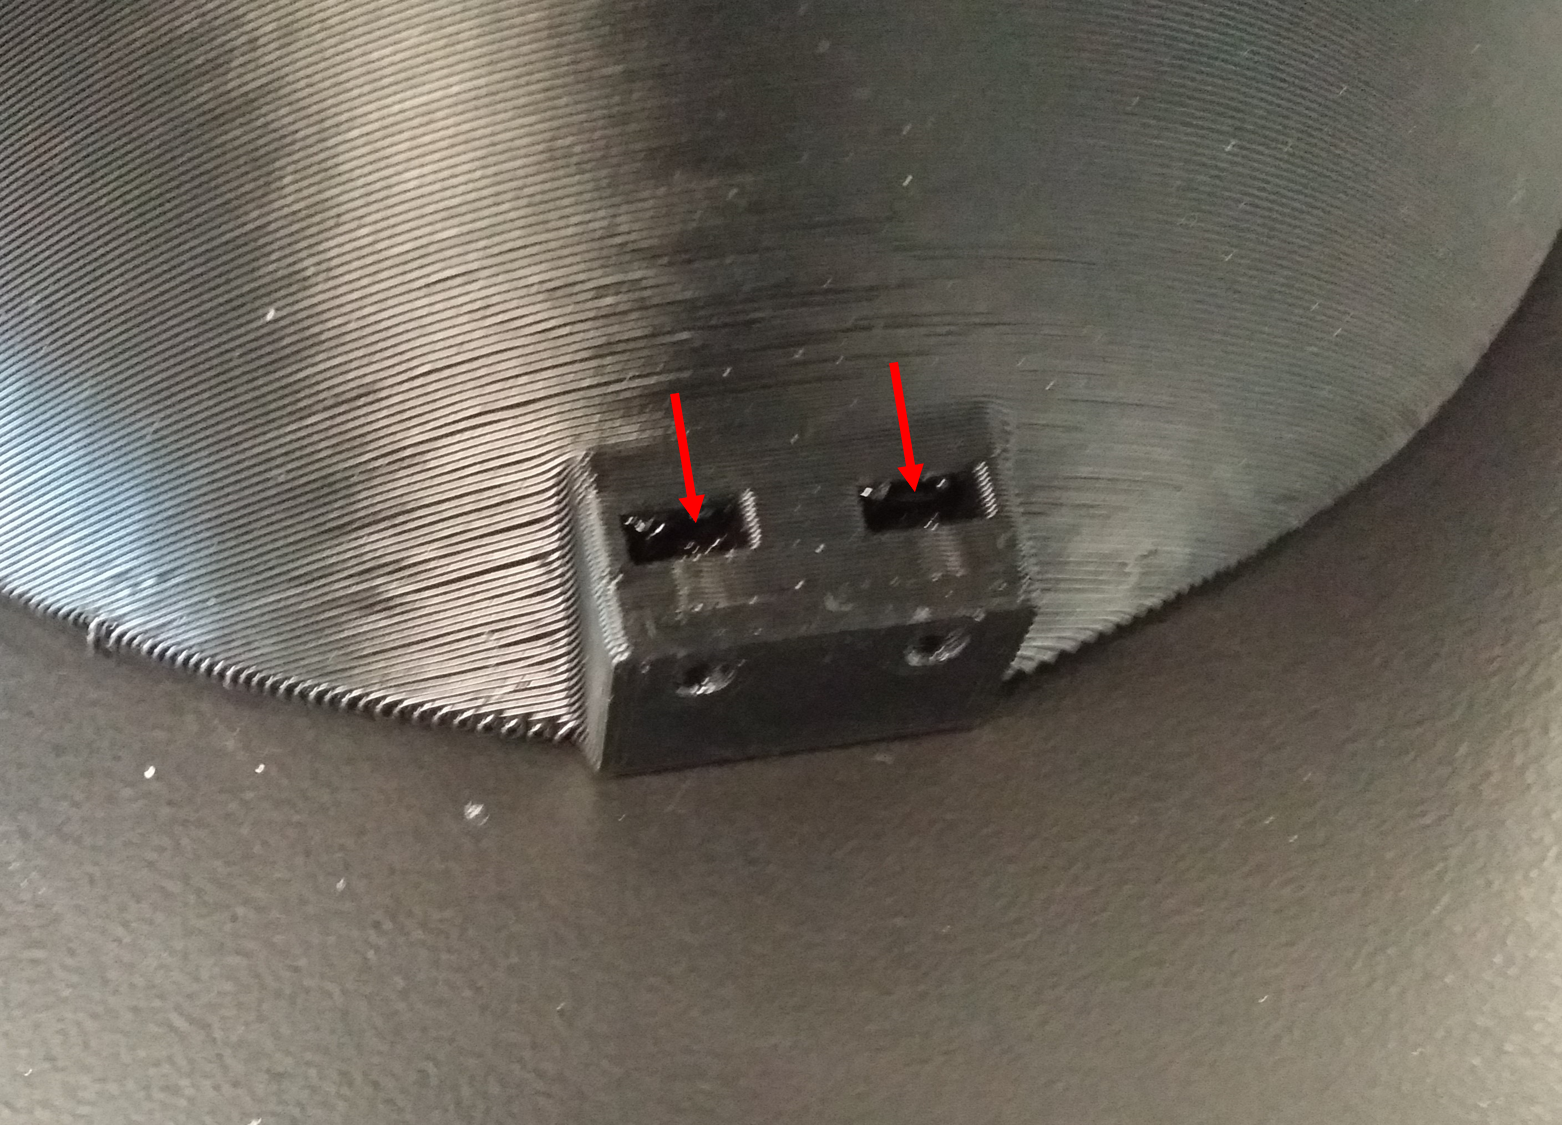
\includegraphics[width=3.6in]{figs/img/assembly/24-reflectorBottomNuts.png}
        \caption{Nuts for Bottom Frame}
        \label{fig:bottomNuts}
    \end{figure}

    \item Place the bottom frame onto the reflectors, with the stop plate pointed upward toward reflector 3. Route the wires through the hole between reflectors 1 and 2 (Fig. \ref{fig:reflectorWireRouting}).
    \begin{figure}[H]
        \centering
        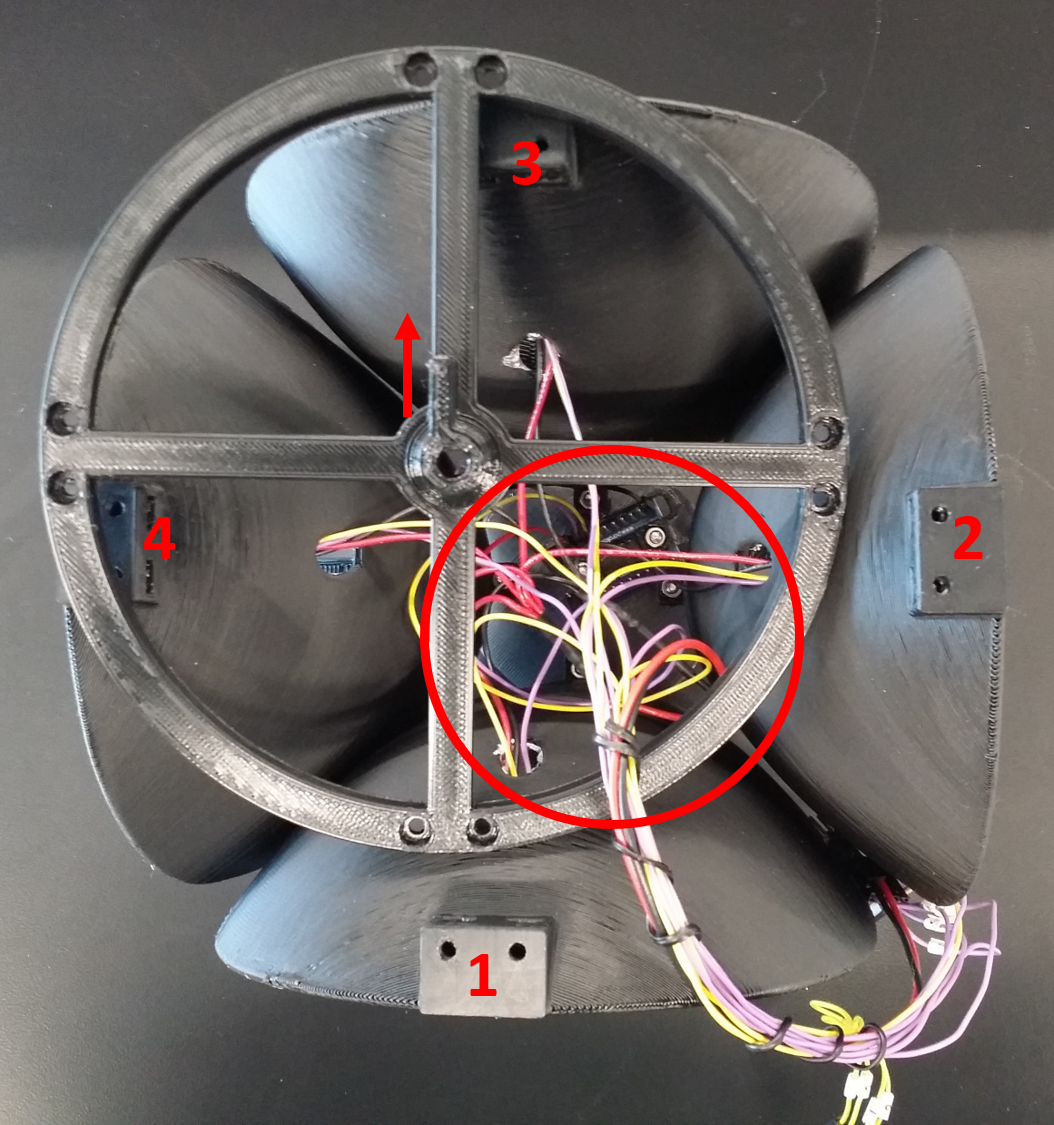
\includegraphics[width=3.9in]{figs/img/assembly/25-reflectorWireRouting.png}
        \caption{Reflector Wire Routing}
        \label{fig:reflectorWireRouting}
    \end{figure}
    \pagebreak

    \item Attach the bottom plate to the reflectors using eight 10mm M3 screws (Fig. \ref{fig:bottomMounting}).
    \begin{figure}[H]
        \centering
        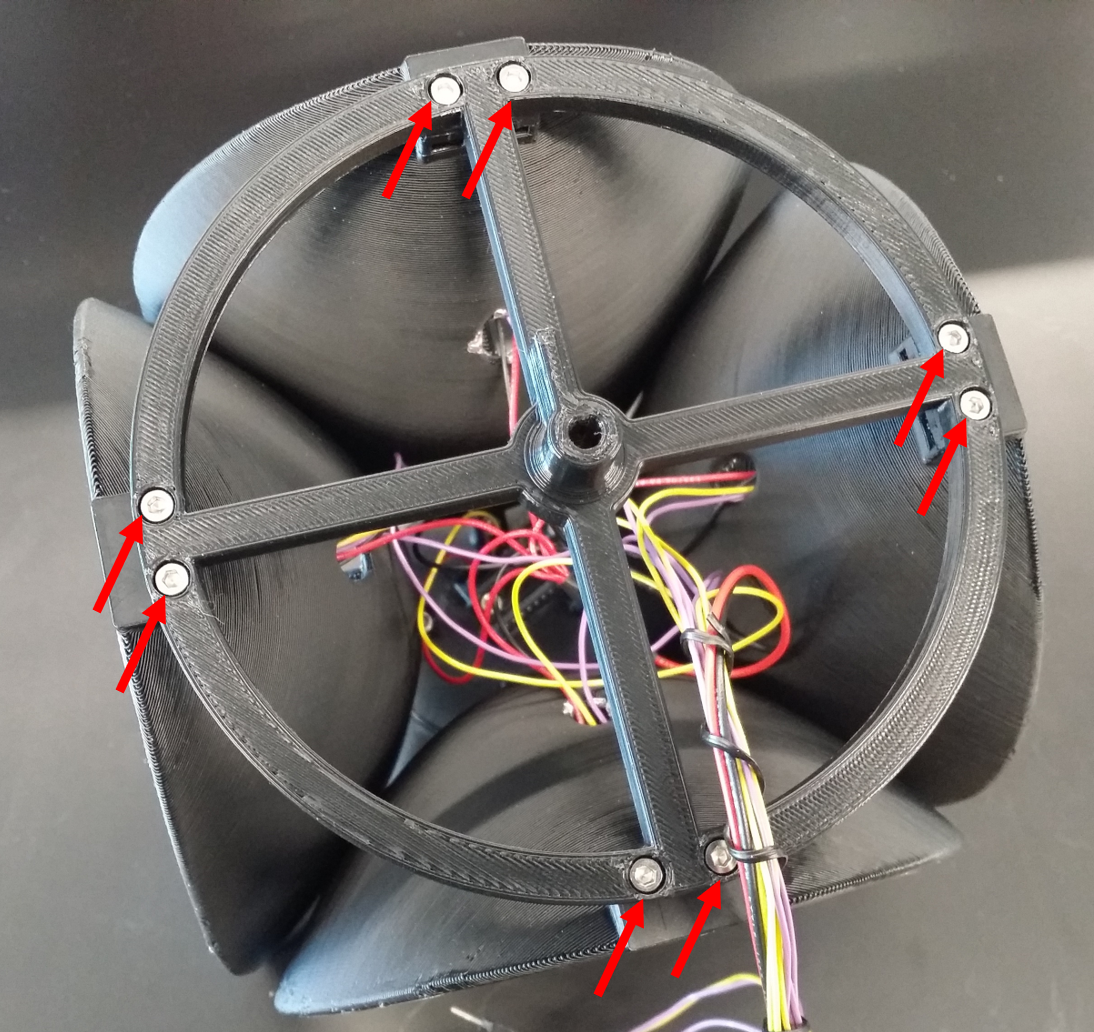
\includegraphics[width=3.6in]{figs/img/assembly/26-reflectorBottomMounting.png}
        \caption{Mounting the Bottom Frame}
        \label{fig:bottomMounting}
    \end{figure}

    \item Insert an XBee into each of the 5 XBee adapter boards (one on top and one in each reflector). Again, make sure that the XBees inside the reflectors are oriented with the antenna on the side toward the reflective surface (Fig. \ref{fig:XBeeInstallation}).
    \begin{figure}[H]
        \centering
        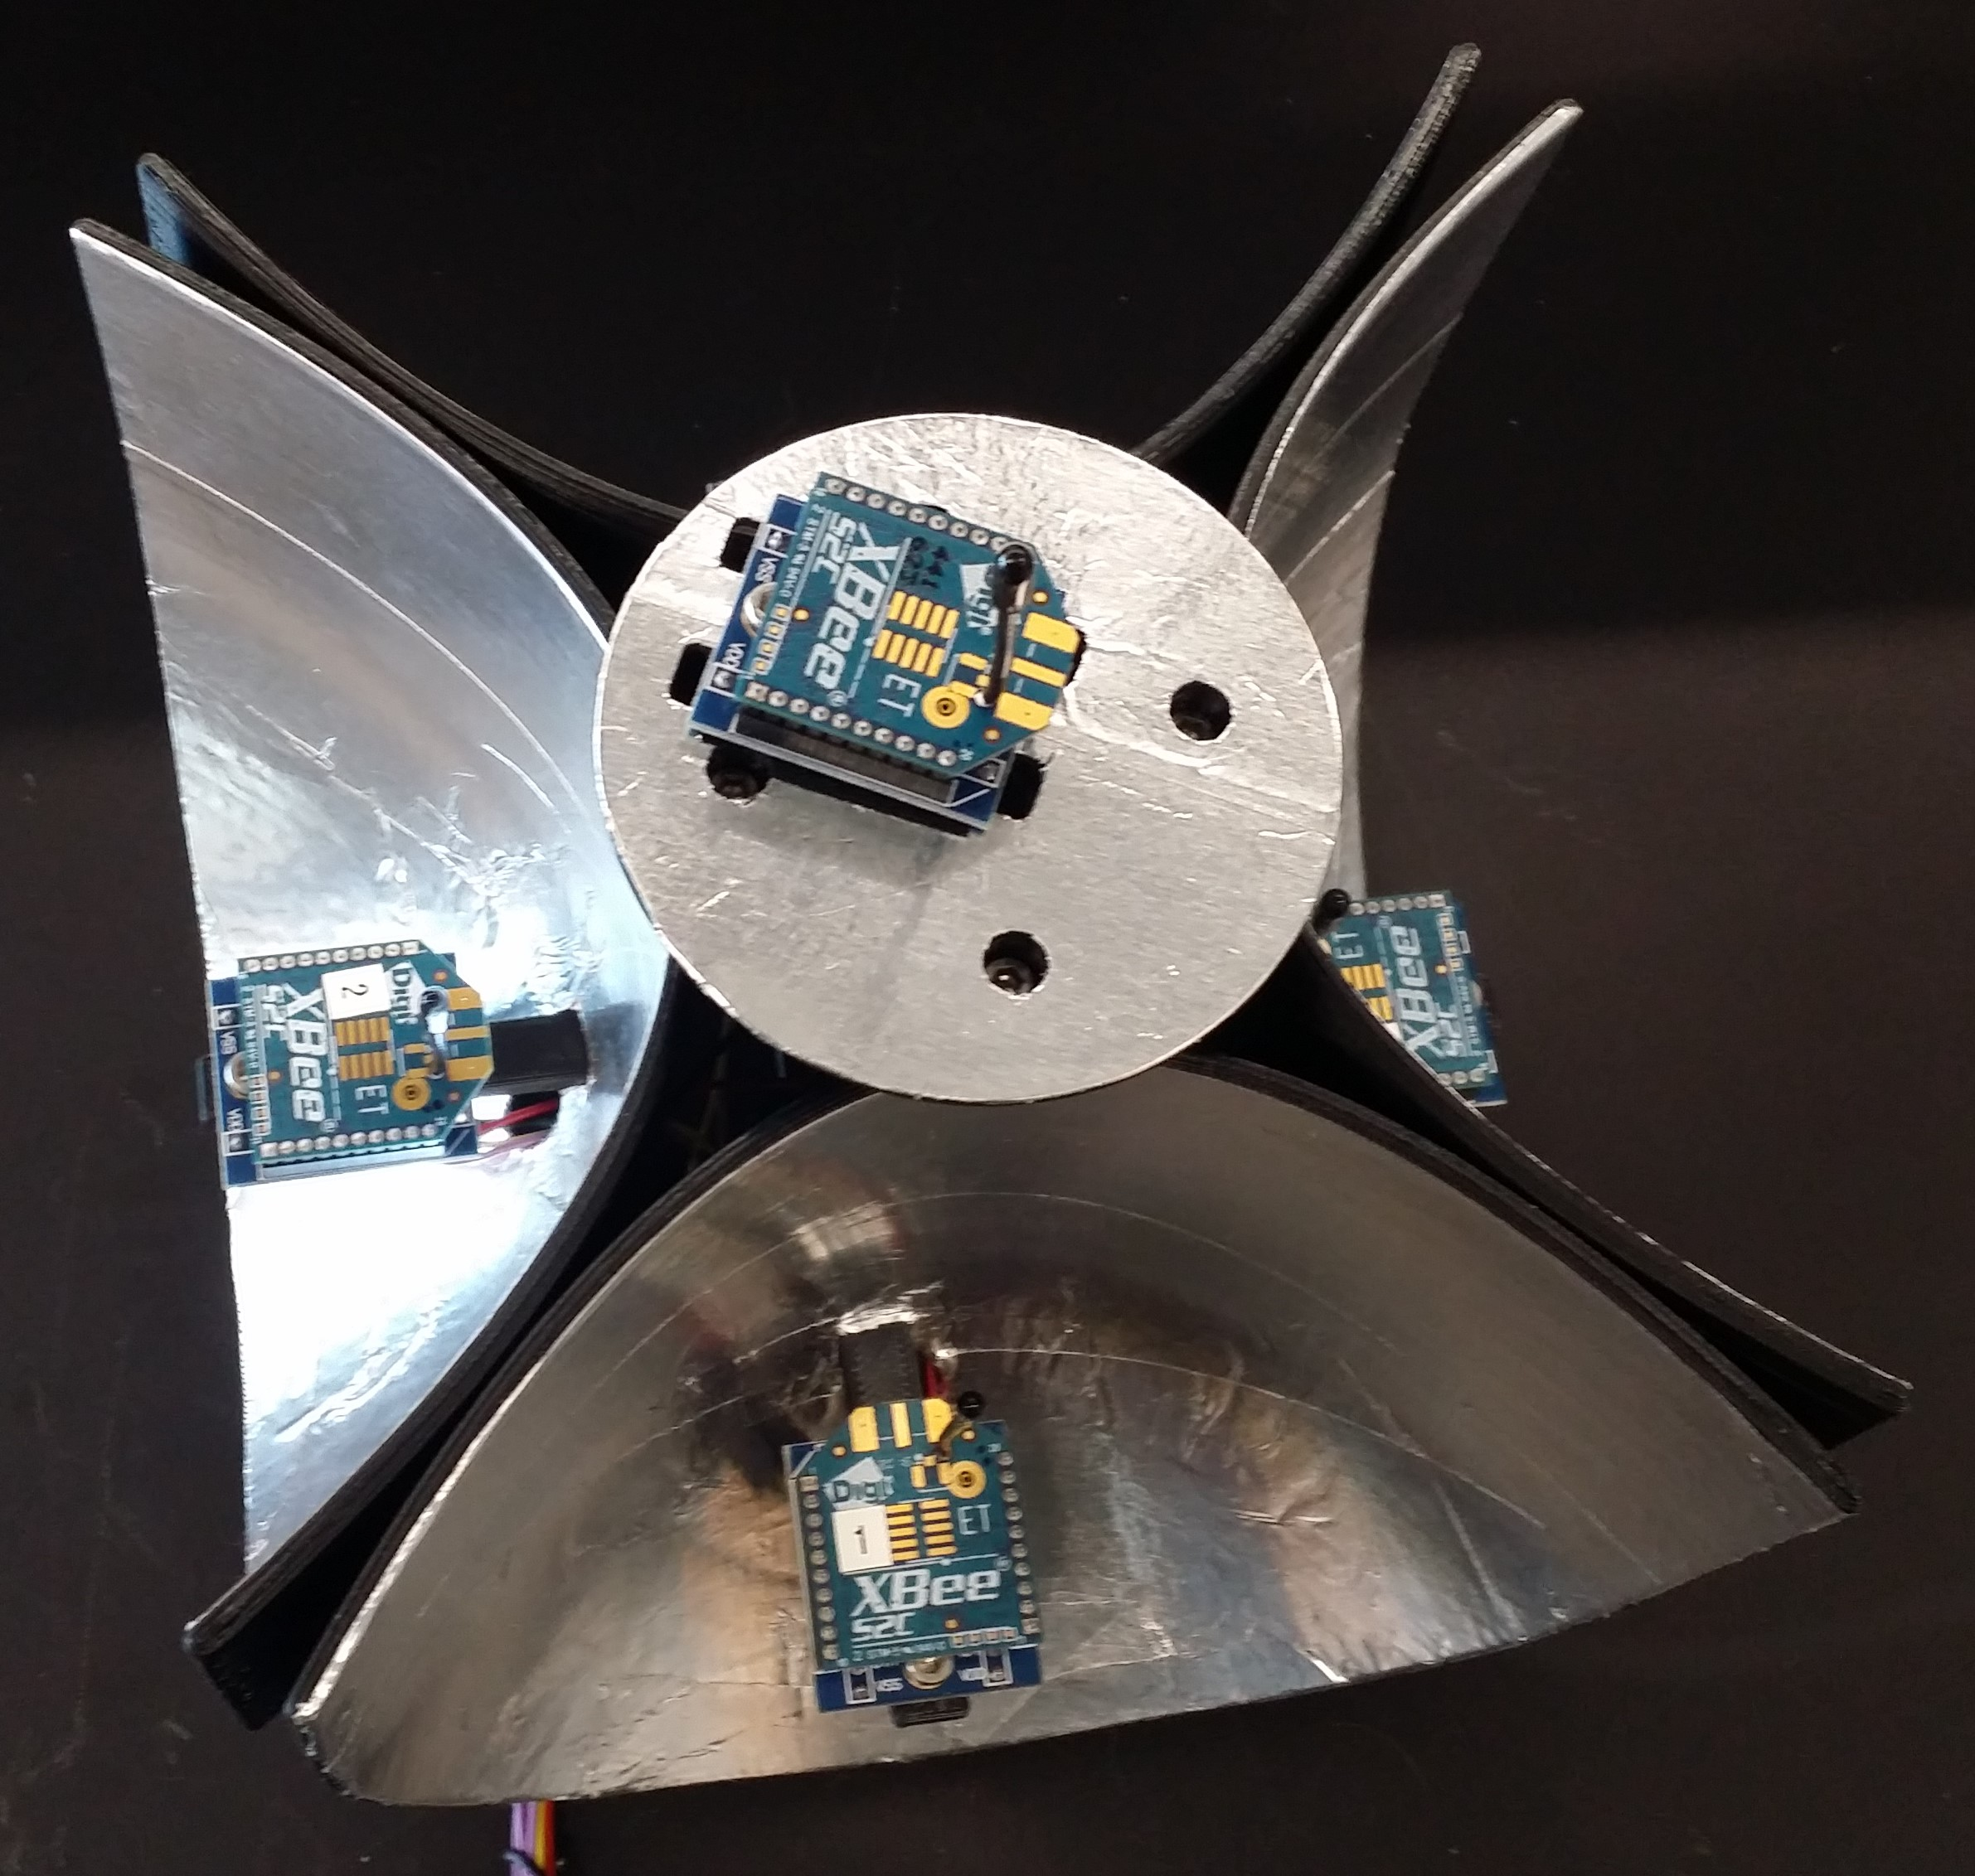
\includegraphics[width=3.6in]{figs/img/assembly/27-XBeeInstallation.jpg}
        \caption{XBee Installation}
        \label{fig:XBeeInstallation}
    \end{figure}
    \pagebreak

    \item Make sure the flat side of the stepper motor shaft is toward the back of the robot. Slide the reflector array onto this motor shaft, making sure the stop plate is pointed toward the back of the robot and is between the two stops on the stepper motor bracket (Fig. \ref{fig:reflectorMounting}).
    \begin{figure}[H]
        \centering
        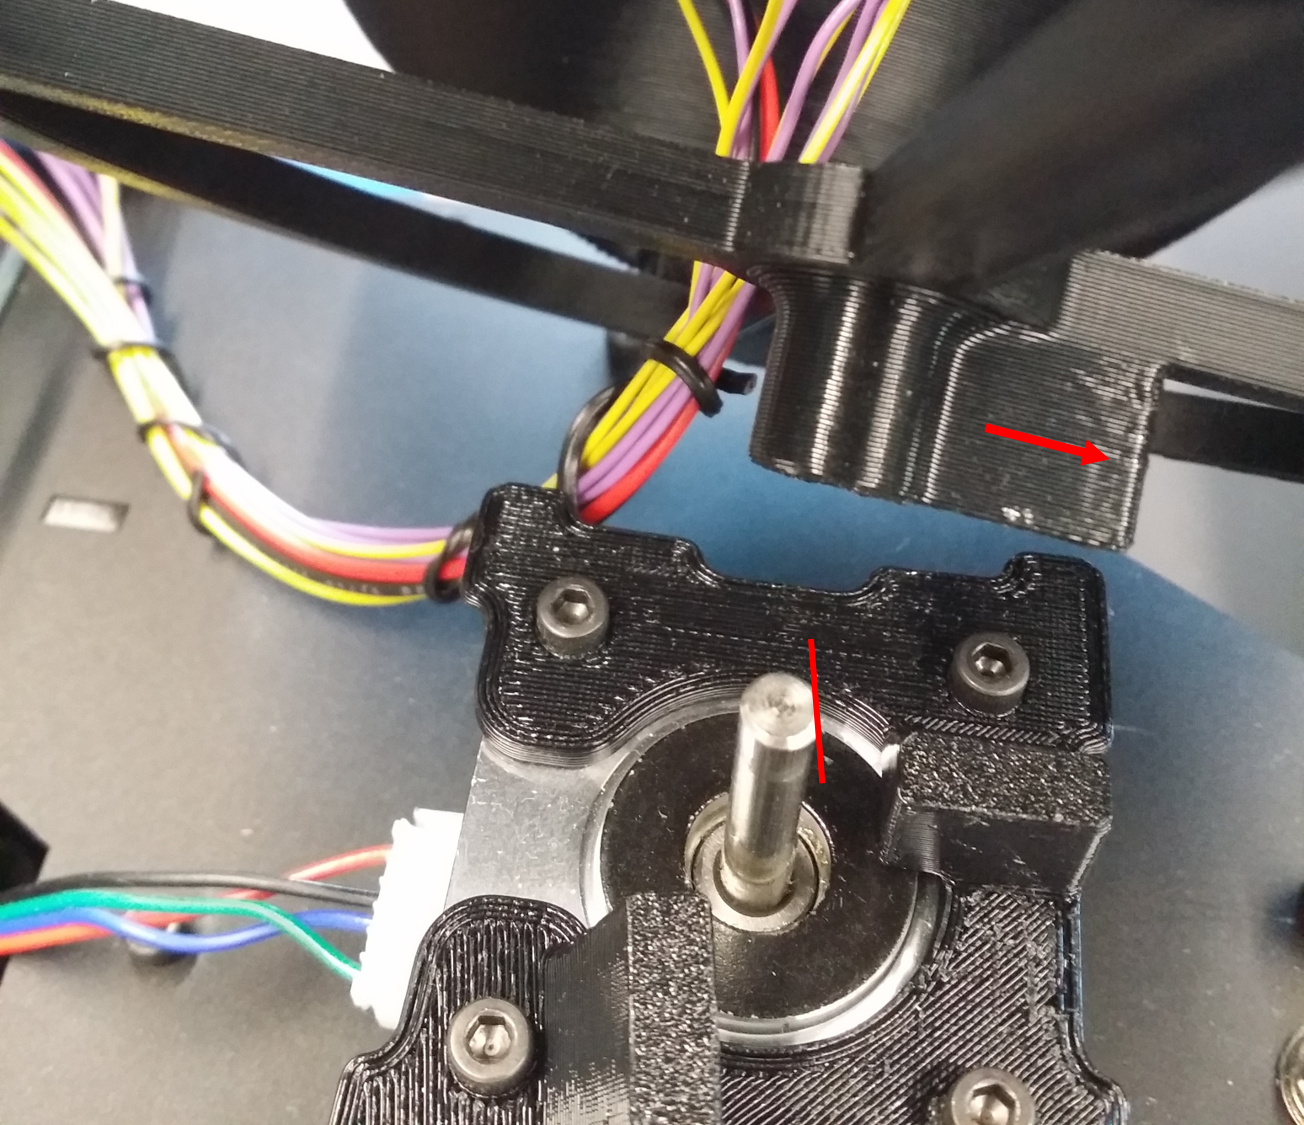
\includegraphics[width=3.8in]{figs/img/assembly/28-reflectorMounting.png}
        \caption{Mounting the Reflectors on the Stepper Motor}
        \label{fig:reflectorMounting}
    \end{figure}

    \item Verify that the stop plate on the reflector array is between the stops on the stepper motor bracket (Fig. \ref{fig:installedReflector})
    \begin{figure}[H]
        \centering
        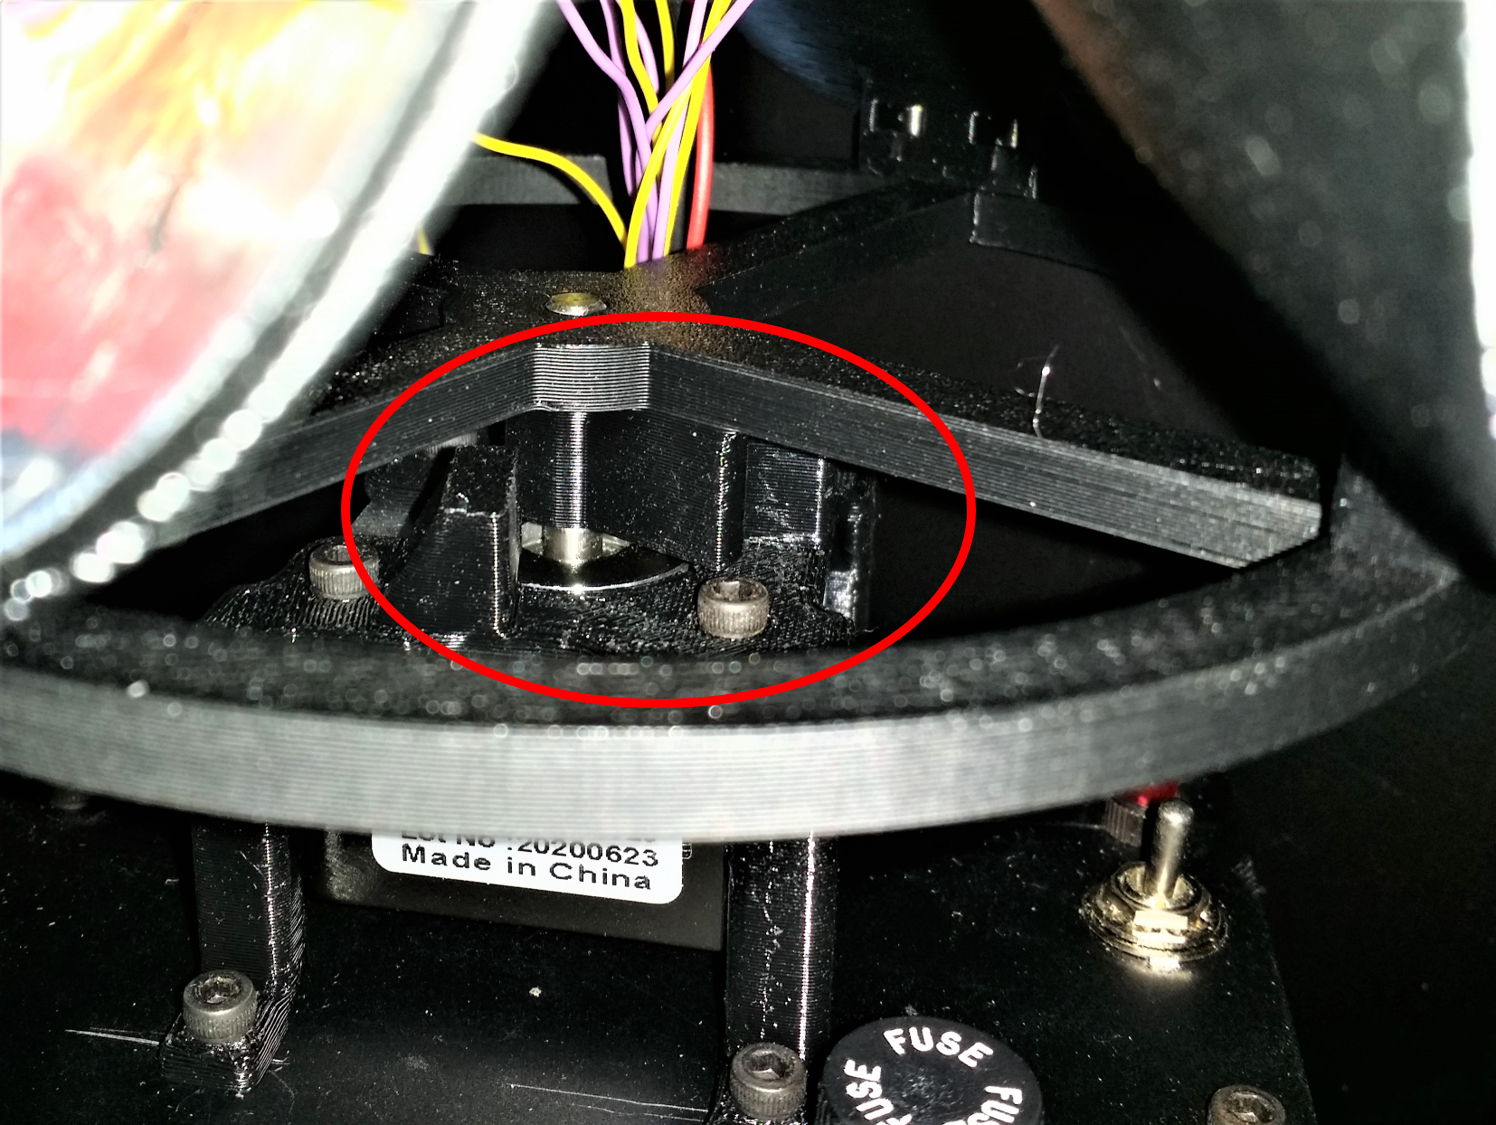
\includegraphics[width=3.8in]{figs/img/assembly/29-installedReflector.png}
        \caption{Reflector Stop Verification}
        \label{fig:installedReflector}
    \end{figure}
    \pagebreak

    \item Connect the reflector to the rest of the system by connecting the power cables to the output of the LM1117 regulator (Fig. \ref{fig:reflectorWiring}, red arrow), the top XBee TX and RX to the UART5 TX and RX (Fig. \ref{fig:reflectorWiring}, blue arrow), the side XBee TX wires to multiplexer pins 10 - 13 (Fig. \ref{fig:reflectorWiring}, purple arrow), and the side XBee RX wires to multiplexer pins 4 - 7 (Fig. \ref{fig:reflectorWiring}, yellow arrow). The side XBees should be connected to the multiplexer in order, with XBee 1 connecting to multiplexer pins 4 and 13.
    \begin{figure}[H]
        \centering
        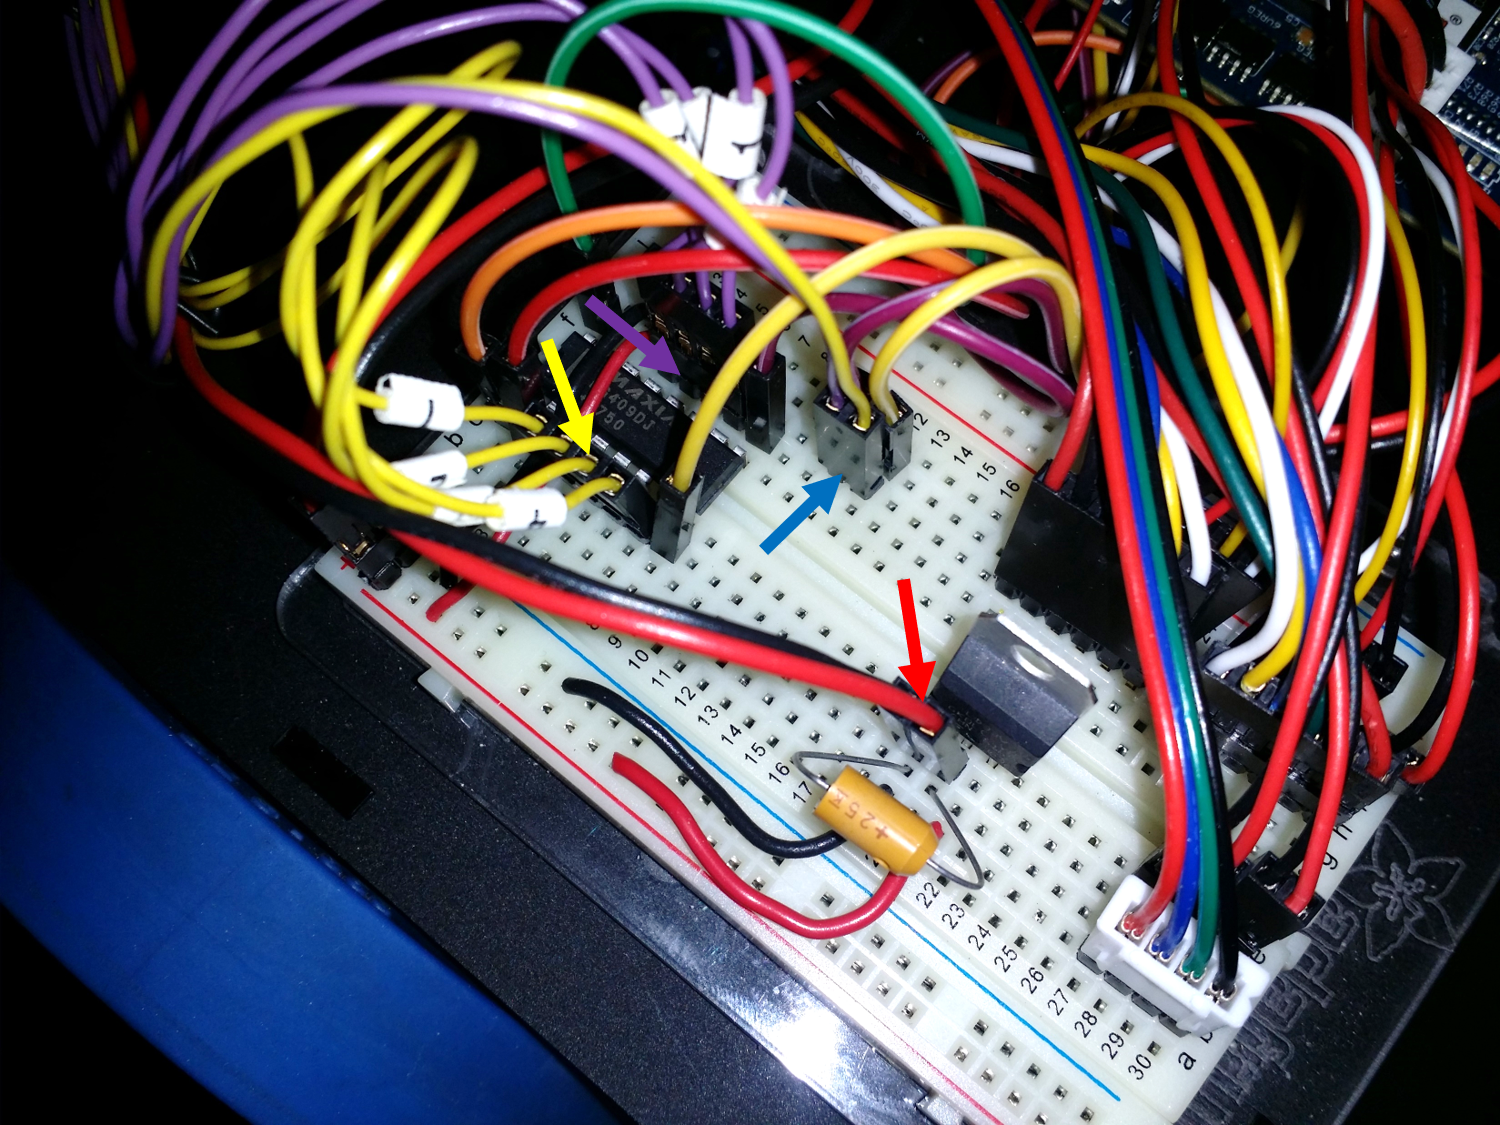
\includegraphics[width=3.4in]{figs/img/assembly/30-reflectorWiring.png}
        \caption{Reflector Wiring}
        \label{fig:reflectorWiring}
    \end{figure}
\end{enumerate}

The robot assembly is complete! The fully assembled robot should look like the one shown in Fig. \ref{fig:assembledRobot}.
\begin{figure}[H]
    \centering
    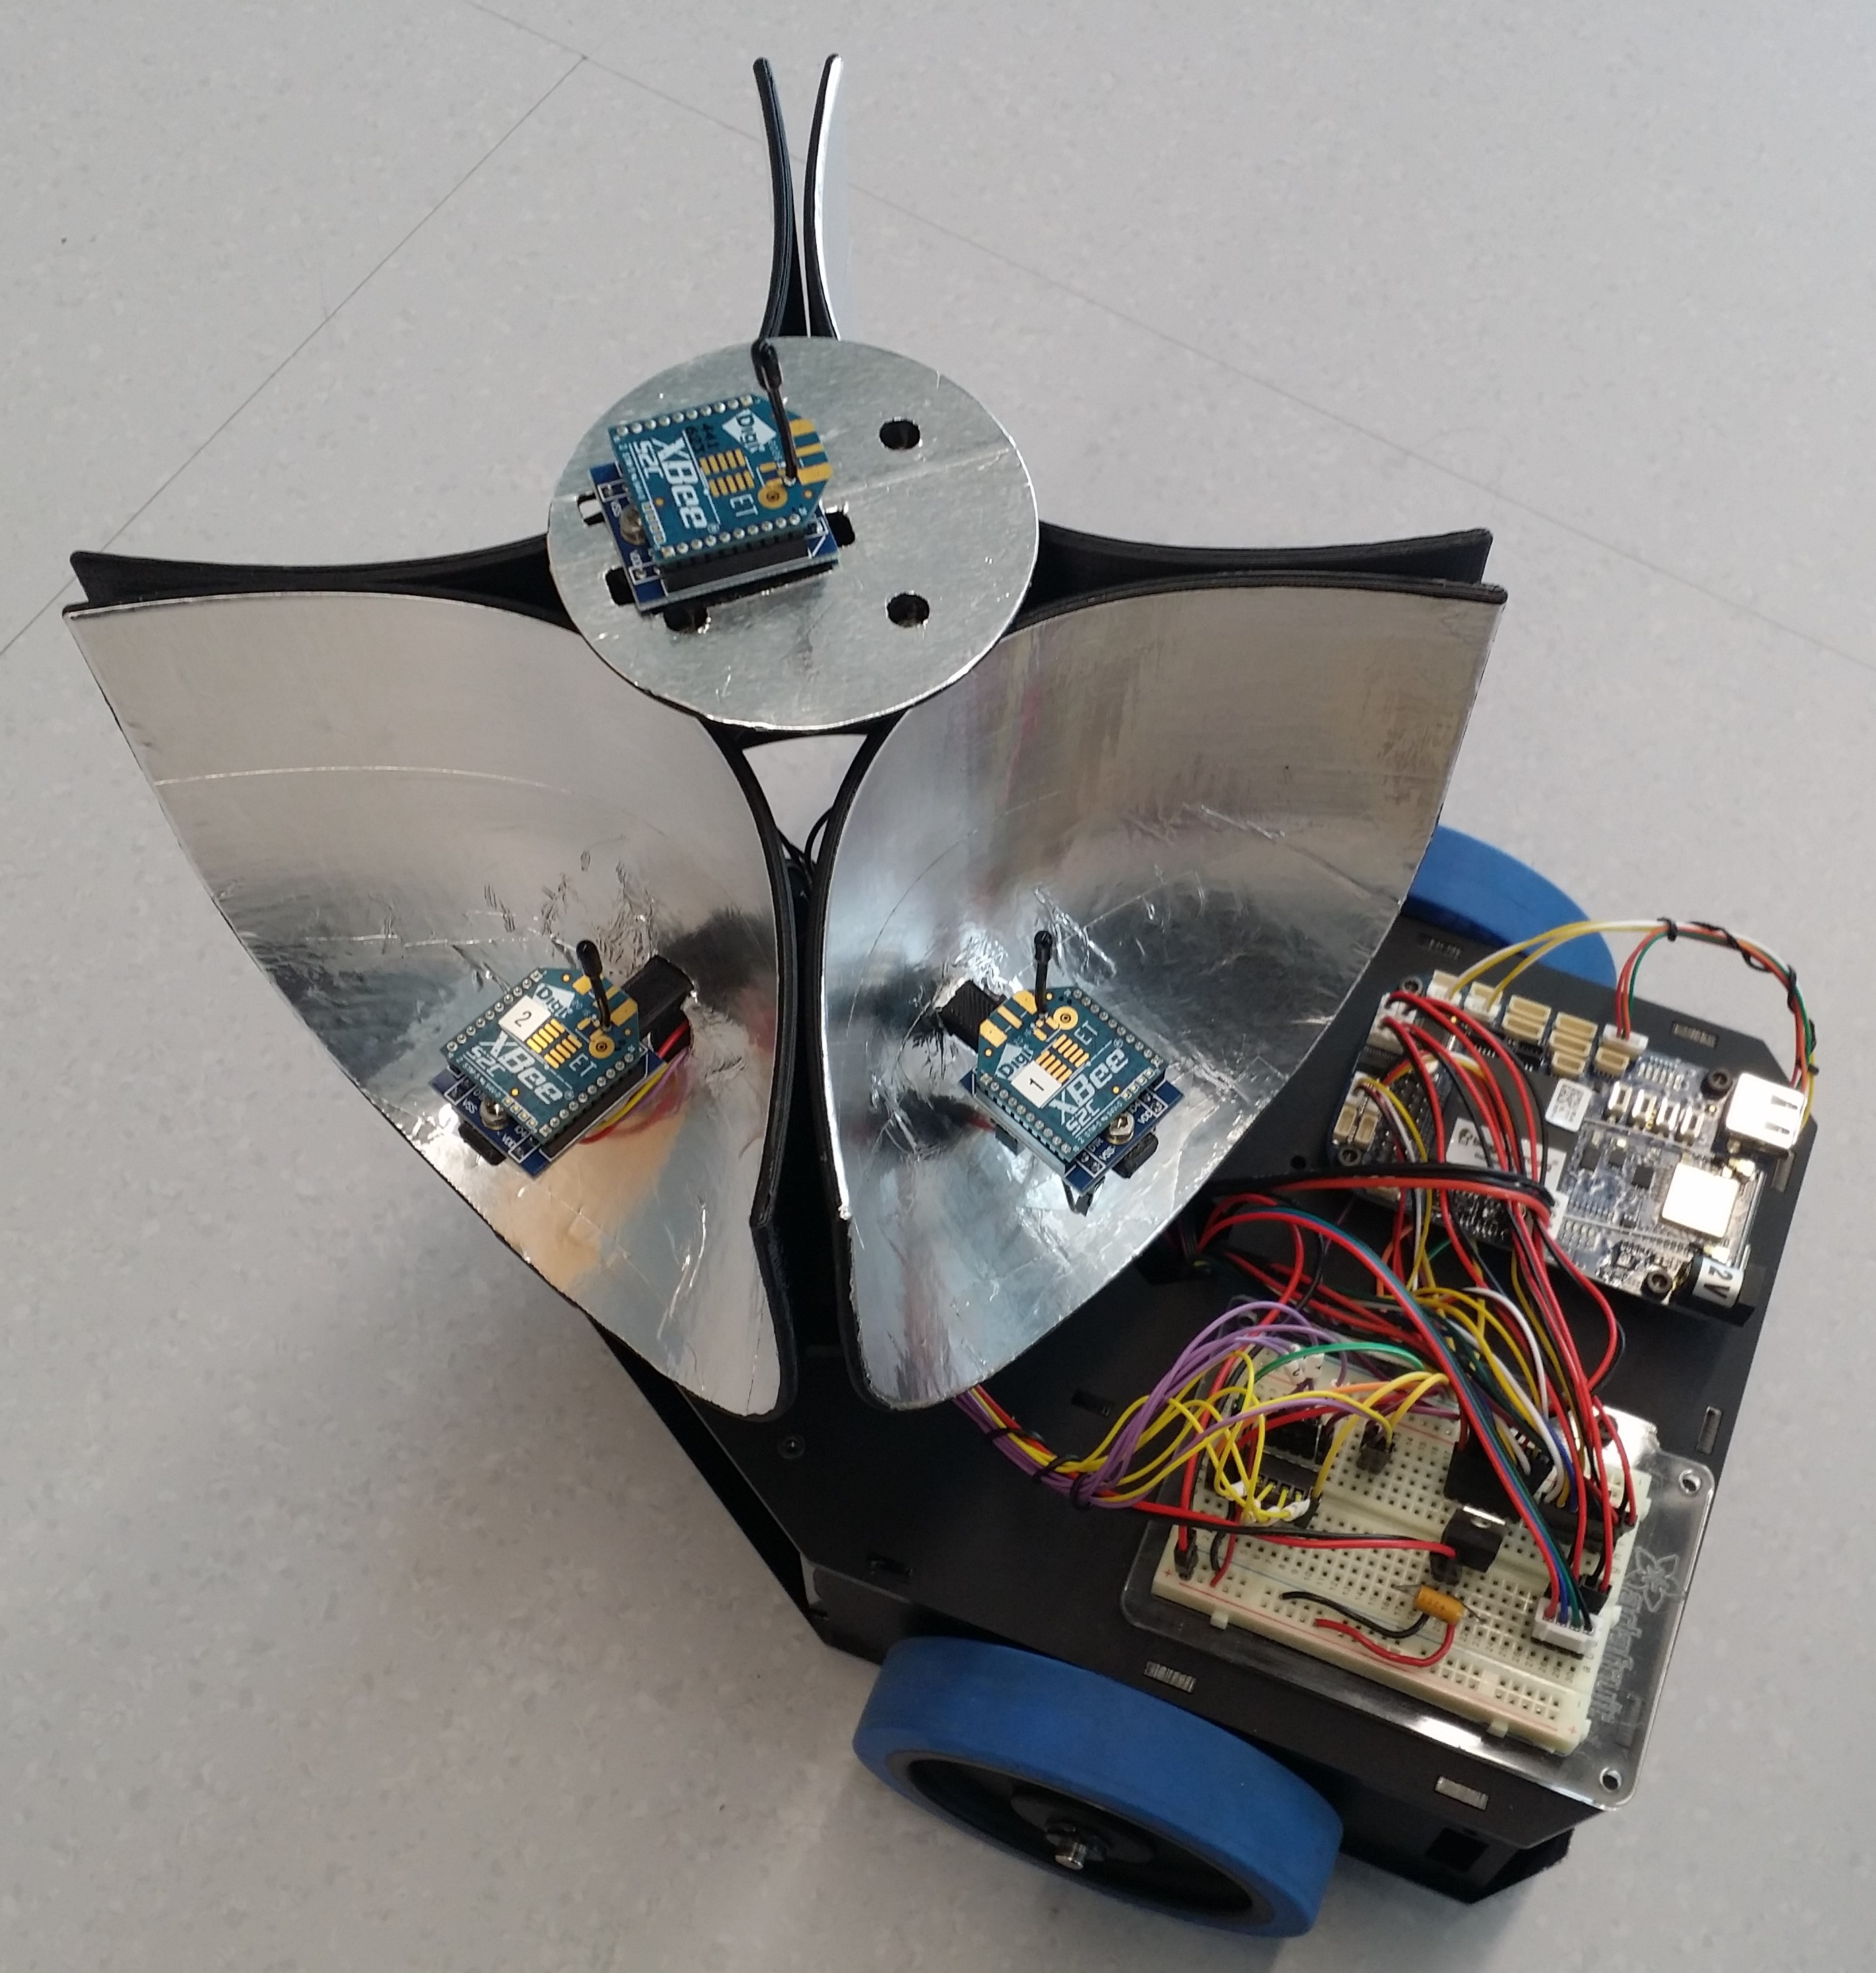
\includegraphics[width=3.4in]{figs/img/assembly/31-assembledRobot.jpg}
    \caption{Assembled Robot}
    \label{fig:assembledRobot}
\end{figure}

%%% Local Variables:
%%% mode: latex
%%% TeX-master: "../finalReport"
%%% End:
